\documentclass[a4paper, 11pt]{article}
\bibliographystyle{alpha}

\title{On the Embeddedness of Minimal Surfaces}
\author{Aris Mercier}
\date{}

%\usepackage[letterpaper, top=2cm, bottom=2cm, left=3.5cm, right=3.5cm, marginparwidth=1.75cm]{geometry}

\usepackage[nottoc,numbib]{tocbibind}

\usepackage{amsmath}
\usepackage{amssymb}
\usepackage{amsfonts}
\usepackage{amsthm}

\usepackage{hyperref}
\hypersetup{
    colorlinks,
    citecolor=blue,
    filecolor=black,
    linkcolor=blue,
    urlcolor=black
}

\usepackage{bbm}
\usepackage{esint}

\usepackage[capitalise, noabbrev]{cleveref}
\usepackage{mathtools}
\usepackage{epigraph}
\usepackage[a4paper]{geometry}
\geometry{includehead, includefoot, left=3cm, right=3cm, top=2cm, bottom=2cm} % head and foot are included in total body so that nothing is printed out of the boundaries of the set margins

%\usepackage{resmes}

\usepackage{tikz}
\usepackage{pgfplots}
\pgfplotsset{compat=1.17}

\theoremstyle{plain}
\newtheorem{theorem}{Theorem}[section] 
\newtheorem{lemma}[theorem]{Lemma}
\newtheorem{proposition}[theorem]{Proposition} 
\newtheorem{corollary}[theorem]{Corollary}
\newtheorem*{claim}{Claim}

\theoremstyle{definition}
\newtheorem{definition}[theorem]{Definition}
\newtheorem{example}[theorem]{Example}
\newtheorem{axiom}{Axiom}
\newtheorem{exercise}[theorem]{Exercise}
\newtheorem*{conjecture}{Conjecture}

\theoremstyle{remark}
\newtheorem*{remark}{Remark} 
\newtheorem{case}{Case}

%------Operators & Commands----------%

\DeclareMathOperator{\diff}{d \!}
\DeclareMathOperator{\diam}{diam}
\DeclareMathOperator{\lip}{Lip}
\DeclareMathOperator{\graph}{graph}

\newcommand{\norm}[1]{\left\lVert#1\right\rVert}


\newcommand{\mres}{\mathrel{\vrule height 1.6ex depth 0pt width 0.13ex\vrule height 0.13ex depth 0pt width 1.3ex}} % <--- Measure Restriction Symbol

\renewcommand{\div}{\text{div}} % <--- Divergence Operator

\numberwithin{equation}{subsection}


%-------------------------------%

\pdfstringdefDisableCommands{
\def\({}
\def\){}
\def\pi{}
}


\begin{document}
\maketitle
\tableofcontents
\newpage

\epigraph{\emph{No one will read this except you and me.}}{― F. Schulze}
\section{Introduction}
In the summer of 2024, I completed a research project at the University of Warwick under the supervision of Professor Felix Schulze. This document contains a write-up of my work during this time.

\cref{Preliminaries} is a brief summary of my background reading in preparation for this project. My main reference has been Leon Simon's \emph{Introduction to Geometric Measure Theory} \cite{Sim18}, which is an updated version of his classic text \emph{Lectures on Geometric Measure Theory}. Parts of this section have also been inspired by \cite{Rin22} and \cite{Mor16}. In an effort to keep this section short, many proofs have been omitted. Instead, citations have been provided throughout, and interested readers are encouraged to consult them for further details.

\cref{Paper} presents an exposition on the research paper \cite{EWW02} by Tobias Ekholm, Brian White, and Daniel Wienholtz. This paper proves a sufficient condition for the embeddedness of minimal surfaces, and moreover imposes certain restrictions on the topology of such surfaces. In this section we examine these results in greater detail, and explore some of their fascinating applications.

The work presented in this document is entirely expository. In particular, I claim absolutely no originality over its contents. I would like to thank all those who inspired and helped me along the way, for the quality of this work would be much poorer without them.

\section{Preliminaries}
\label{Preliminaries}

\subsection{Preliminaries from Measure Theory}

\subsubsection{Covering Theorems}

We begin by exploring a class of results known as \emph{covering theorems}. The main idea is as follows: starting from a family of covering sets, we wish to select a subfamily with some control on the overlap of the sets. In particular, the sets might be pairwise disjoint or almost disjoint (in the measure-theoretic sense). This may seem similar to the notion of compactness, which we now recall:

\begin{definition}
A topological space \(T\) is \emph{compact} if every open cover contains a finite subcover.
\end{definition}

A simple covering theorem is the following:

\begin{proposition}
Let \(A \subset \mathbb{R}^{n}\) be a bounded set, and fix \(r > 0\). Then there are finitely many elements \(x_{1},\ldots,x_{N}\) such that
\begin{equation}
A \subset \bigcup_{k=1}^{N}B_{r}(x_{k}),
\end{equation}
and every \(x \in A\) is contained in at most \(3^{n}\) of the balls \(B_{r}(x_{k})\).
\end{proposition}

Note that the first part of the proposition follows immediately by compactness,\footnote{Even if A is not compact, it is contained in a compact set.} so the essence of a covering result is controlling the overlap of the balls.

A significant generalisation of the previous result is given by the \emph{Besicovich covering theorem}:

\begin{theorem}[Besicovitch Covering Theorem]
Suppose \(\mathcal{F}\) is a collection of closed balls in \(\mathbb{R}^n\) such that the set \(A\) of their centres is bounded. Then for some \(N\), depending on \(n\), there exist sub-collections \(\mathcal{F}_1,\ldots,\mathcal{F}_N \subset \mathcal{F}\), each consisting of pairwise disjoint balls, such that \(\bigcup_{i=1}^{N}\mathcal{F}_i\) still covers \(A\). That is,
\begin{equation}
A \subset \bigcup_{i=1}^{N}\bigg(\bigcup_{F \in \mathcal{F}_i}F\bigg).
\end{equation}
In particular, there is a finite or countable cover of \(A\), consisting of closed balls in \(\mathcal{F}\), such that every point of \(\mathbb{R}^n\) is contained in at most \(N\) of these balls.
\end{theorem}

Next, we present an improved version of the classical \emph{Vitali covering theorem}. Recall that, given a set \(A \subset \mathbb{R}^{n}\), a \emph{fine cover} of \(A\) is a family \(\mathcal{F}\) of closed balls such that every point in \(A\) is contained in a ball in \(\mathcal{F}\) of arbitrarily small radius.

\begin{theorem}[Besicovich--Vitali Covering Theorem]
Let \(A \subset \mathbb{R}^{n}\) be a bounded Borel set and let \(\mathcal{F}\) be a fine cover of \(A\). For every Radon measure \(\mu : \mathcal{B}(\mathbb{R}^{n}) \rightarrow V\), there is a disjoint and countable subfamily \(\mathcal{F}' \subset \mathcal{F}\) which covers \(A\) \(\mu\)-almost everywhere. Here \((V, \norm{\cdot})\) is a normed vector space.
\end{theorem}

We emphasise that the corresponding claim with open balls instead of closed balls is false. Consider the following example:

\begin{example}
Let \(A \coloneq \{0\} \cup \left\{\frac{1}{n} : n \in \mathbb{N}\right\}\), and define the fine cover \(\mathcal{F}\) of \(A\) to be
\begin{equation}
\mathcal{F} \coloneq \left\{\left(-\frac{1}{m}, \frac{1}{m}\right) : m \in \mathbb{N}\right\} \cup \left\{\left(\frac{1}{n}-\frac{1}{m}, \frac{1}{n} + \frac{1}{m}\right) : m, n \in \mathbb{N}, m > n \right\}.
\end{equation}

Let \(\mu\) be any positive Radon measure with \(\mu(\{a\}) > 0\) for all \(a \in A\). Then there is no finite or countable subcover of \(\mathcal{F}\) that covers \(\mu\)-almost all of \(A\). On the other hand, if we use closed intervals in the definition of \(\mathcal{F}\) then a finite subcover exists, consisting of the single interval \([-1,1]\).
\end{example}

\subsubsection{Hausdorff Measure}

Suppose \((X,d)\) is a metric space, and let
\begin{equation}
\omega_k \coloneq \frac{\pi^{k/2}}{\Gamma\left(\frac{k}{2}+1\right)}, \ k \geqslant 0,
\end{equation}
where \(\Gamma\) is Euler's Gamma function. If \(k \in \mathbb{N}\), this is the volume of a \(k\)-dimensional unit ball in \(\mathbb{R}^k\).

For \(k \geqslant 0\), we define the \(k\)-dimensional Hausdorff outer measure as the limit
\begin{equation}
\label{Hausdorff_Measure}
\mathcal{H}^k(A) \coloneq \lim_{\delta \downarrow 0} \mathcal{H}^{k}_{\delta}(A), \ A \subset X,
\end{equation}
where, for each \(\delta > 0\), \(\mathcal{H}^{k}_{\delta}\) is defined by taking  \(\mathcal{H}^{k}_{\delta}(\varnothing) \coloneq 0\) and
\begin{equation}
\label{Hausdorff_Measure_delta}
\mathcal{H}^{k}_{\delta}(A) \coloneq \inf \sum_{i=1}^{\infty} \omega_k\left(\frac{\diam C_i}{2}\right)^{k}
\end{equation}
for any non-empty \(A \subset X\). The infimum is taken over all countable collections \(C_1, C_2, \ldots\) of subsets of \(X\) such that \(\diam C_i < \delta\) and \(A \subset \bigcup_{i=1}^{\infty} C_i\). If no such collection exists, the right-hand side of \eqref{Hausdorff_Measure_delta} is taken to be \(+\infty\). The limit in \eqref{Hausdorff_Measure} always exists, since \(\mathcal{H}^{k}_{\delta}(A)\) is a decreasing function of \(\delta\).

Note also that \(\mathcal{H}^0\) is exactly the counting measure.

\begin{theorem}[Isodiametric Inequality]
Let \(A \subset \mathbb{R}^n\). Then
\begin{equation}
\mathcal{L}^n(A) \leqslant \omega_{n}\left(\frac{\diam A}{2}\right)^{n}.
\end{equation}
\end{theorem}
Thus, among all sets \(A \subset \mathbb{R}^n\) with a given diameter \(\lambda\), the ball with diameter \(\lambda\) has the largest \(\mathcal{L}^n\)-measure.

\begin{theorem}
For every \(\mathcal{L}^{n}\)-measurable \(A \subset \mathbb{R}^n\) and every \(\delta > 0\), we have that
\begin{equation}
\mathcal{L}^{n}(A) = \mathcal{H}^{n}(A) = \mathcal{H}^{n}_{\delta}(A).
\end{equation}
\end{theorem}

That is to say, the Hausdorff measure agrees with the Lebesgue measure on sets of integer dimension.

\subsubsection{Densities}

Suppose \((X,d)\) is a metric space. We first want to introduce the notion of the \(n\)-dimensional density of a measure \(\mu\) on \(X\). For any outer measure \(\mu\) on \(X\), any subset \(A \subset X\), and any point \(x \in X\), we define the \(n\)-dimensional upper and lower densities by
\begin{align}
\Theta^{*n}(\mu, A, x) &\coloneq \limsup_{\rho \downarrow 0} \frac{\mu(A \cap B_{\rho}(x))}{\omega_{n} \rho^{n}} \\
\Theta^{n}_{*}(\mu, A, x) &\coloneq \liminf_{\rho \downarrow 0} \frac{\mu(A \cap B_{\rho}(x))}{\omega_{n} \rho^{n}}
\end{align}
In the case that \(A = X\), we simply write \(\Theta^{*n}(\mu, x)\) and \(\Theta^{n}_{*}(\mu, x)\) to denote these quantities. Thus we have that \(\Theta^{*n}(\mu, A, x) = \Theta^{*n}(\mu \mres A, x)\) and \(\Theta^{n}_{*}(\mu, A, x) = \Theta^{n}_{*}(\mu \mres A, x)\).

If \(\Theta^{*n}(\mu, A, x) = \Theta^{n}_{*}(\mu, A, x)\), then we call this common value the \emph{density}, and denote it by \(\Theta^{n}(\mu, A, x)\).

It turns out that appropriate information about the upper density allows us to relate the measure \(\mu\) to the Hausdorff measure \(\mathcal{H}^{n}\). In particular, we have the following comparison theorem:

\begin{theorem}
Let \(\mu\) be an outer measure on \(X\) such that all Borel sets are measurable. Suppose also that \(t \geqslant 0\) and \(A_{1} \subset A_{2} \subset X\). Then
\begin{equation}
\Theta^{*n}(\mu, A_{2}, x) \geqslant t \ \forall x \in A_{1} \implies t\mathcal{H}^{n}(A_{1}) \leqslant \mu(A_{2}).
\end{equation}
\end{theorem}

Importantly, we are not assuming that the sets \(A_{1}\) and \(A_{2}\) are \(\mu\)-measurable.
The curious reader might wonder why the Hausdorff measure appears in the above result. Note the factor of \(\omega_{n}\rho^{n}\) in the definition of the upper density, and recall that this is nothing more than the Hausdorff measure of the ball of radius \(\rho\) in \(\mathbb{R}^{n}\).

As a corollary, we can now prove the following \emph{uppper density theorem}:

\begin{theorem}[Upper Density Theorem]
If \(\mu\) is an outer measure on \(X\) such that all Borel sets are measurable, and if \(A\) is a \(\mu\)-measurable subset of X with \(\mu(A) < \infty\), then
\begin{equation}
\Theta^{*n}(\mu, A, x) = 0
\end{equation}
for \(\mathcal{H}^{n}\)-almost every \(x \in X \setminus A\).
\end{theorem}

\begin{corollary}
If \(A \subset \mathbb{R}^{n}\) is \(\mathcal{L}^{n}\)-measurable, then the density \(\Theta^{n}(\mathcal{L}^{n}, A, x)\) exists for \(\mathcal{L}^{n}\)-a.e. \(x \in \mathbb{R}^{n}\). Moreover, \(\Theta^{n}(\mathcal{L}^{n}, A, x) = \mathbbm{1}_{A}(x)\) for \(\mathcal{L}^{n}\)-a.e. \(x \in \mathbb{R}^{n}\).
\end{corollary}

We also introduce the particular notion of \emph{density at infinity}. For this, readers should first familiarise themselves with the \emph{extended monotonicity theorem} \ref{Extended Monotonicity}. Consider now a properly immersed minimal surface \(M \in \mathbb{R}^{n}\) without boundary. Then the density ratio \(\Theta(M, p, r)\) increases with \(r\), and so converges to a (potentially infinite) limit as \(r \rightarrow \infty\). Moreover, we have the inclusion
\begin{equation}
B(p,r) \subset B(q, r + \vert p-q \vert),
\end{equation}
from which it follows that the limit is independent of the point p, and can therefore be written unambiguously as \(\Theta(M)\). We call this value the \emph{density of} M \emph{at infinity}.

\subsubsection{Differentiation Theorems}

We wish to extend the comparison and upper density theorems from the previous section to a more general setting. For this, we consider the density of a Borel regular measure \(\nu\) with respect to another Borel regular measure \(\mu\). We will always assume that \(\mu\) is locally finite. That is, for all \(x \in X\) there exists a \(\rho > 0\) such that \(\mu(B_{\rho}(x)) < \infty\).

In this case, the \emph{upper density} \(\Theta^{*\mu}(\nu, x)\) of \(\nu\) with respect to \(\mu\) at a point \(x \in X\) is defined by
\begin{equation}
\Theta^{*\mu}(\nu, x) \coloneq
\begin{cases}
\limsup\limits_{\smash{\rho \downarrow 0}} \frac{\nu(B_{\rho}(x))}{\mu(B_{\rho}(x))} & \text{for } x \in \operatorname{supp} \mu \cap \operatorname{supp} \nu, \\
\infty & \text{for } x \in \operatorname{supp} \nu \setminus \operatorname{supp} \mu, \\
0 & \text{for } x \notin \operatorname{supp} \nu.
\end{cases}
\end{equation}
Note that \(\Theta^{*n}(\mu, x)\) is a special case of \(\Theta^{*\mu}(\nu, x)\) where \(X = \mathbb{R}^{n}\) and \(\mu = \mathcal{L}^{n}\).

The \emph{lower density} of \(\nu\) with respect to \(\mu\) is defined analogously. If these two agree, then this common value is known as the \emph{density}, and is denoted by \(\Theta^{\mu}(\nu, x)\).

We will also require a few preliminary definitions. The \emph{support} of a measure \(\mu\) on \(X\), denoted \(\operatorname{supp} \mu\), is the set of all points \(x \in X\) such that \(\mu(U) > 0\) for all open neighbourhoods \(U\) of \(x\). For a measure \(\mu : \mathcal{B}(X) \rightarrow V\), the \emph{total variation measure} \(\norm{\mu}\) is defined as follows: for all Borel sets \(A \in \mathcal{B}(X)\), let
\begin{equation}
\norm{\mu}(A) \coloneq \sup\bigg\{\sum_{n=1}^{\infty} \norm{\mu(A_{n})} : (A_{n})_{n} \text{ is a partition of } X \text{ by Borel sets.}\bigg\}.
\end{equation}

\begin{definition}
Suppose  \((X, \mathcal{B}(X))\) is a measurable space, and consider two measures \(\mu : \mathcal{B}(X) \rightarrow [0, +\infty]\) and \(\nu : \mathcal{B}(X) \rightarrow V\), where \((V, \norm{\cdot})\) is a normed vector space. We say that \(\nu\) is \emph{absolutely continuous} with respect to \(\mu\) if, denoted \(\nu \ll \mu\), if \(\norm{\nu}(A) = 0\) for all \(A\) such that \(\mu(A) = 0\).
\end{definition}

The total variation is required in the above definition because the measure \(\nu\) is vector-valued.

\begin{theorem}[Besicovich Differentiation Theorem]
Let \(\mu : \mathcal{B}(\mathbb{R}^{n}) \rightarrow [0, +\infty]\) and \(\nu : \mathcal{B}(\mathbb{R}^{n}) \rightarrow V\), where \((V, \norm{\cdot})\) is a normed vector space. Then for \(\mu\)-almost every \(x \in \operatorname{supp}\mu\), the ``blow-up quotient'' limit
\begin{equation}
\label{Radon--Nikodym Derivative}
\frac{\diff\nu}{\diff\mu}(x) \coloneq \lim_{\rho \downarrow 0} \frac{\nu(B_{\rho}(x))}{\mu(B_{\rho}(x))}
\end{equation}
exists in \(V\), and \(\nu\) has the \emph{Radon--Nikodym decomposition}
\begin{equation}
\nu = \frac{\diff\nu}{\diff\mu}\mu + \nu^{s}.
\end{equation}
The \emph{singular part} \(\nu^{s} : \mathcal{B}(\mathbb{R}^{n}) \rightarrow V\) is given by \(\nu^{s} \coloneq \nu \mres E\), where
\begin{equation}
E \coloneq (\mathbb{R}^{n} \setminus \operatorname{supp}\mu) \cup \bigg\{x \in \operatorname{supp}\mu : \lim_{\rho \downarrow 0} \frac{\norm{\nu}(B_{\rho}(x))}{\mu(B_{\rho}(x))} = \infty \bigg\}.
\end{equation}
\end{theorem}

\begin{theorem}[Radon--Nikodym Theorem]
Let \(\mu : \mathcal{B}(\mathbb{R}^{n}) \rightarrow [0, +\infty]\) and \(\nu : \mathcal{B}(\mathbb{R}^{n}) \rightarrow V\), where \((V, \norm{\cdot})\) is a normed vector space, and assume that \(\nu\) is \emph{absolutely continuous} with respect to \(\mu\). Then
\begin{equation}
\nu = \frac{\diff\nu}{\diff\mu} \mu,
\end{equation}
where \(\frac{\diff\nu}{\diff\mu}\) is the \emph{Radon--Nikodym derivative}, defined in \eqref{Radon--Nikodym Derivative}.
\end{theorem}

\begin{theorem}[Lebesgue Differentiation Theorem]
Let \(\mu : \mathcal{B}(\mathbb{R}^{n}) \rightarrow [0, +\infty]\), and suppose \(f \in L^{1}(\mathbb{R}^{n}, \mathcal{B}(\mathbb{R}^{n}), \mu)\). Then
\begin{equation}
\lim_{\rho \downarrow 0} \fint_{B_{\rho}(x_{0})}\vert f(x) - f(x_{0}) \vert \diff\mu(x) = 0
\end{equation}
for \(\mu\)-almost every \(x_{0} \in \mathbb{R}^{n}\). That is, \(\mu\)-almost every \(x_{0} \in \mathbb{R}^{n}\) is a \emph{Lebesgue point} of \(f\) with respect to \(\mu\).
\end{theorem}

\begin{corollary}
Let \(\mu : \mathcal{B}(\mathbb{R}^{n}) \rightarrow [0, +\infty]\). Then \(\mu\)-almost every \(x_{0} \in \operatorname{supp} \mu\) is a \emph{density point} of \(\mu\), that is,
\begin{equation}
\lim_{\rho \downarrow 0} \frac{\mu(B_{\rho}(x_{0}) \cap \operatorname{supp} \mu)}{\mu(B_{\rho}(x_{0}))} = 1.
\end{equation}
\end{corollary}

\subsection{Preliminaries from Analysis}

\subsubsection{Lipschitz Functions}

Let \((X,d)\) be a metric space, and recall that a function \(f \vcentcolon X \rightarrow \mathbb{R}\) is said to be  \emph{Lipschitz} if there exists \(L < \infty\) such that
\begin{equation}
\left|f(x) - f(y)\right| \leqslant L d(x,y)
\end{equation}
for all \(x,y \in X\). The least such \(L\) is called the Lipschitz constant and is denoted by \(\lip f\).

Lipschitz functions satisfy the following basic extension theorem:

\begin{theorem}
\label{Lipschitz_Extension_Theorem}
If \(A\) is a non-empty subset of \(X\) and \(f \vcentcolon A \rightarrow \mathbb{R}\) is Lipschitz, then there exists a Lipschitz \(\overline{f} \vcentcolon X \rightarrow \mathbb{R}\) such that \(\lip \overline{f} = \lip f\) and \(\overline{f}\vert_A = f\).
\end{theorem}

Moreover, the set on which a Lipschitz function fails to be differentiable cannot, in some sense, be very large. More formally, we have the following important result:

\begin{theorem}[{Rademacher, \cite[Section 2.1]{Sim18}}]
If \(f\) is Lipschitz on \(\mathbb{R}^n\), then \(f\) is differentiable \(\mathcal{L}^n\)-almost everywhere. That is, the gradient \(\nabla f(x_0) = (D_1 f(x_0), \ldots, D_n f(x_0))\) exists and
\begin{equation}
\lim_{x \rightarrow x_0} \frac{f(x) - f(x_0) - \nabla f(x_0) \cdot (x-x_0)}{|x-x_0|} = 0
\end{equation}
for \(\mathcal{L}^n\)-a.e. \(x \in \mathbb{R}^n\).
\end{theorem}

Following a common theme in real analysis, we aim to approximate Lipschitz functions by functions which exhibit higher regularity. This can be done by the following approximation theorem:


\begin{theorem}
Suppose \(f \vcentcolon \mathbb{R}^n \rightarrow \mathbb{R}\) is Lipschitz. Then for each \(\varepsilon > 0\) there exists a function \(g \in C^1(\mathbb{R}^n)\) such that
\begin{equation}
\mathcal{L}^n(\{x \in \mathbb{R}^n \vcentcolon f(x) \neq g(x)\} \cup \{x \in \mathbb{R}^n \vcentcolon \nabla f(x) \neq \nabla g(x)\}) < \varepsilon.
\end{equation}
\end{theorem}

The proof makes use of Whitney's Extension Theorem.

\subsubsection{The Area and Coarea Formul\ae}

We now establish two fundamental results in geometric measure theory, namely the area and coarea formul\ae. The former is a generalisation of the classical change-of-variables formula that one encounters in multivariable analysis. The latter is a generalisation of Fubini's theorem from flat slices to level sets of a Lipschitz map.

Let \(f \vcentcolon \mathbb{R}^n \rightarrow \mathbb{R}^k\) be differentiable at \(x \in \mathbb{R}^n\). If \(n \leqslant k\), define the \(n\)-dimensional Jacobian of \(f\) at \(x\) by
\begin{equation}
\mathbf{J}_{n}f(x) \coloneq \sqrt{\det(Df(x)^{T}Df(x))}.
\end{equation}
If \(n \geqslant k\), define the \(k\)-dimensional Jacobian of \(f\) at \(x\) by
\begin{equation}
\mathbf{J}_{k}f(x) \coloneq \sqrt{\det(Df(x)Df(x)^{T})}.
\end{equation}
Note that if \(n = k\), then both definitions agree and reduce to
\begin{equation}
\mathbf{J}_{n}f(x) = \vert\det Df(x)\vert,
\end{equation}
which is the factor in the classical transformation formula for integrals.

The first version of the area formula concerns maps defined on the flat space \(\mathbb{R}^n\). We will encounter another, more general version, in the following chapters.

\begin{theorem}[Area Formula]
Let \(f \vcentcolon \mathbb{R}^n \rightarrow \mathbb{R}^k\) be Lipschitz, with \(n \leqslant k\). Then, for every \(\mathcal{L}^n\)-measurable map \(g \vcentcolon \mathbb{R}^n \rightarrow \mathbb{R}\) it holds that
\begin{equation}
\int_{\mathbb{R}^{n}}g(x)\mathbf{J}_{n}f(x)\diff\mathcal{L}^{n}(x) = \int_{\mathbb{R}^{k}}\sum_{x \in f^{-1}(y)}g(x)\diff \mathcal{H}^{n}(y).
\end{equation}
In particular, if \(A \subset \mathbb{R}^{n}\) is \(\mathcal{L}^{n}\)-measurable, then
\begin{equation}
\int_{A}\mathbf{J}_{n}f(x)\diff\mathcal{L}^{n}(x) = \int_{\mathbb{R}^{k}}\mathcal{H}^{0}(A \cap f^{-1}(y))\diff \mathcal{H}^{n}(y),
\end{equation}
and if, moreover, \(f\) is injective, then
\begin{equation}
\label{Area_Formula_3}
\int_{A}\mathbf{J}_{n}f(x)\diff\mathcal{L}^{n}(x) = \mathcal{H}^{n}(f(A)).
\end{equation}
\end{theorem}
By Rademacher's theorem we know that \(f\) is differentiable \(\mathcal{L}^{n}\)-almost everywhere, and so \(\mathbf{J}_{n}f(x)\) exists \(\mathcal{L}^{n}\)-almost everywhere. Hence the above integrals are well-defined.

\begin{example}[Space Curves]
Using the area formula, we first check that the \(\mathcal{H}^1\) measure agrees with the usual arc-length measure for \(C^1\) curves in \(\mathbb{R}^{k}\). In fact, if \(\gamma : [a,b] \rightarrow \mathbb{R}^{k}\) is an injective \(C^1\) map, then its Jacobian is just \(\sqrt{|\dot{\gamma}|^2} = |\dot{\gamma}|\), so the area formula \eqref{Area_Formula_3} gives
\begin{equation}
\mathcal{H}^1(\gamma([a,b])) = \int_{a}^{b}|\dot{\gamma}(x)|\diff x,
\end{equation}
as required.
\end{example}

\begin{example}[Submanifolds of \(\mathbb{R}^{n+k}\)]
\label{Area_Formula_Submanifolds}
\end{example}

\begin{example}[\(n\)-dimensional graphs in \(\mathbb{R}^{n+1}\)]
If \(U\) is a domain in \(\mathbb{R}^n\), and if \(M = \graph u\), where \(u \in C(U ; \mathbb{R})\), then \(M\) is globally represented by the map \(x \overset{f}{\longmapsto} (x, u(x))\). In this case,
\begin{equation}
\mathbf{J}_{n}f(x) = \sqrt{\det(D_{i}f \cdot D_{j}f)} = \sqrt{\det(\delta_{ij} + D_i u D_j u)} = \sqrt{1 + |Du|^2},
\end{equation}
so \(\mathcal{H}^n(M) = \int_U\sqrt{1+ |Du|^2} \diff x\).
\end{example}

\begin{theorem}[Coarea Formula]
Let \(f \vcentcolon \mathbb{R}^{n} \rightarrow \mathbb{R}^{k}\) be Lipschitz, with \(n \geqslant k\). Then, for every \(\mathcal{L}^{n}\)-measurable map \(g \vcentcolon \mathbb{R}^n \rightarrow \mathbb{R}\) it holds that
\begin{equation}
\int_{\mathbb{R}^{n}}g(x)\mathbf{J}_{k}f(x)\diff \mathcal{L}^{n}(x) = \int_{\mathbb{R}^{k}}\int_{f^{-1}(y)}g(x)\diff \mathcal{H}^{n-k}(x)\diff \mathcal{L}^{k}(y).
\end{equation}
In particular, if \(A \subset \mathbb{R}^{n}\) is \(\mathcal{L}^{n}\)-measurable, then
\begin{equation}
\int_{A}\mathbf{J}_{k}f(x)\diff \mathcal{L}^{n}(x) = \int_{\mathbb{R}^{k}}\mathcal{H}^{n-k}(A \cap f^{-1}(y))\diff \mathcal{L}^{k}(y).
\end{equation}
\end{theorem}

\begin{remark}
The fibre \(f^{-1}(y)\) is not necessarily a smooth \((n-k)\)-dimensional submanifold of \(\mathbb{R}^{n}\), even if \(f \in C^{\infty}(\mathbb{R}^{n})\). In fact it need not be a manifold at all. Consider for example the function \(f \vcentcolon \mathbb{R}^{2} \rightarrow \mathbb{R}\) defined by \(f(x_{1}, x_{2}) \coloneq x_{2}^{2} - (x_{1}^3-3x_{1})\). Then \(f \in C^{\infty}(\mathbb{R}^2)\), but the fibre \(f^{-1}(2)\) shown in \cref{Fig: self-intersecting curve} is not a submanifold of \(\mathbb{R}^{2}\).
\end{remark}

\begin{figure}
\begin{center}
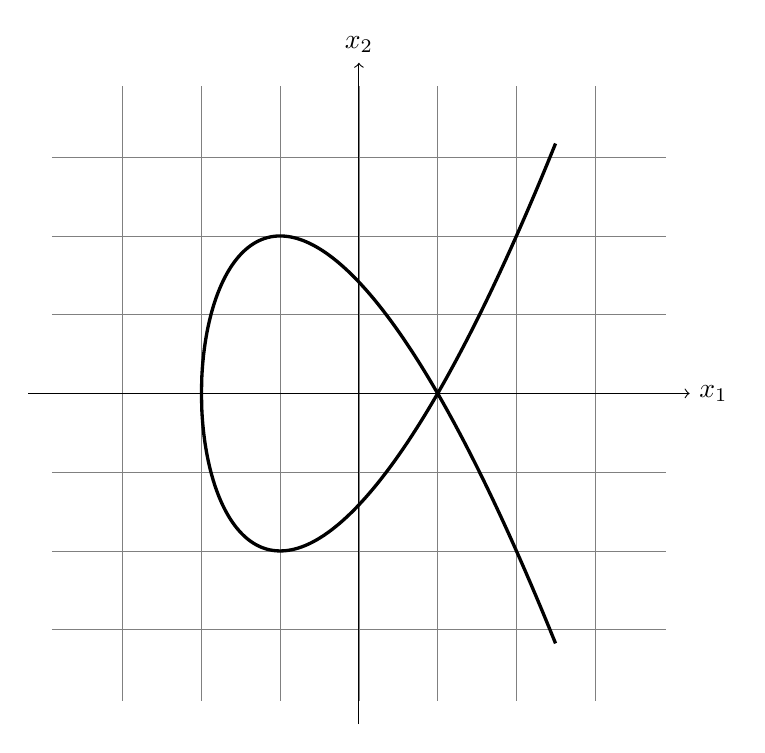
\begin{tikzpicture}
  \draw[very thin,color=gray] (-3.9,-3.9) grid (3.9,3.9);
  \draw[->] (-4.2,0) -- (4.2,0) node[right] {$x_{1}$};
  \draw[->] (0,-4.2) -- (0,4.2) node[above] {$x_{2}$};
  \draw[very thick, domain=-2:2.5, smooth, variable=\x, samples = 1000] plot ({\x}, {sqrt(\x^3 - 3*\x + 2)});
  \draw[very thick, domain=-2:2.5, smooth, variable=\x, samples = 1000] plot ({\x}, {-sqrt(\x^3 - 3*\x + 2)});
\end{tikzpicture}
\end{center}
\vspace{-5ex}
\caption{A self-intersecting curve in \(\mathbb{R}^{2}\).}
\label{Fig: self-intersecting curve}
\end{figure}


\begin{example}[Polar Coordinates]
\label{Polar_Coordinates}
Let \(g \vcentcolon \mathbb{R}^{n} \rightarrow \mathbb{R}\) be \(\mathcal{L}^{n}\)-measurable. Then
\begin{equation}
\int_{\mathbb{R}^{n}}g(x)\diff \mathcal{L}^{n}(x) = \int_{0}^{\infty}\int_{\partial B(r)}g(x)\diff\mathcal{H}^{n-1}(x)\diff r,
\end{equation}
or, alternatively,
\begin{equation}
\frac{\!\diff}{\diff r}\int_{B(r)}g(x)\diff \mathcal{L}^{n}(x) = \int_{\partial B(r)}g(x)\diff\mathcal{H}^{n-1}(x).
\end{equation}
This follows from applying the coarea formula to the modulus function \(f \vcentcolon \mathbb{R}^{n} \rightarrow \mathbb{R}\), given by \(f(x) \coloneq |x|\). In particular, we note that \(\nabla f(x) = \frac{x}{|x|}\) and \(\mathbf{J}_{1}f(x) = 1\) for all \(x \neq 0\).
\end{example}

\subsection{Countably \(n\)-Rectifiable Sets}

A set \(M \subset \mathbb{R}^{n+k}\) is said to be countably \(n\)-rectifiable if
\begin{equation}
M \subset M_0 \cup \bigg(\bigcup_{i=1}^{\infty}F_i(\mathbb{R}^n)\bigg),
\end{equation}
where \(\mathcal{H}^{n}(M_0) = 0\) and \(F_i \vcentcolon \mathbb{R}^{n} \rightarrow \mathbb{R}^{n+k}\) are Lipschitz functions for \(i = 1,2,\ldots\).

Note that by the extension theorem \ref{Lipschitz_Extension_Theorem}, this is equivalent to saying
\begin{equation}
M = M_0 \cup \bigg(\bigcup_{i=1}^{\infty}F_i(A_i)\bigg),
\end{equation}
where \(\mathcal{H}^{n}(M_0) = 0\), \(A_i \subset \mathbb{R}^{n}\) and \(F_i \vcentcolon A_i \rightarrow \mathbb{R}^{n+k}\) are Lipschitz functions for \(i = 1,2,\ldots\). More importantly, we have the following lemma:

\begin{lemma}
\label{Rectifiable_iff_submanifoldCover}
A set \(M \subset \mathbb{R}^{n+k}\) is countably \(n\)-rectifiable if and only if \(M \subset \bigcup_{i=0}^{\infty}N_i\), where \(\mathcal{H}^{n}(N_0) = 0\), and where \(N_i\) is an \(n\)-dimensional embedded \(C^1\) submanifold of \(\mathbb{R}^{n+k}\) for each \(i = 1,2,\ldots\).
\end{lemma}

We now want to give an important characterization of countably \(n\)-rectifiable sets in terms of \emph{approximate tangent spaces}, which we first define:

\begin{definition}
Let \(M\) be an \(\mathcal{H}^n\)-measurable subset of \(\mathbb{R}^{n+k}\) such that \(\mathcal{H}^{n}(M \cap K) < \infty\) for each compact \(K \subset \mathbb{R}^{n+k}\). For \(x \in \mathbb{R}^{n+k}\), we say that an \(n\)-dimensional linear subspace \(\pi \subset \mathbb{R}^{n+k}\) is an approximate tangent space to \(M\) at \(x\) if
\begin{equation}
\lim_{\lambda \downarrow 0} \int_{\lambda^{-1}(M-x)}\varphi(y) \diff \mathcal{H}^{n}(y) = \int_{\pi}\varphi(y)\diff \mathcal{H}^{n}(y)
\end{equation}
for each \(\varphi \in C_{c}(\mathbb{R}^{n+k})\).
\end{definition}
If such a subspace exists then it is unique, and we denote it by \(T_x M\). It turns out that the rectifiability of \(M\) is equivalent to the existence \(\mathcal{H}^{n}\)-a.e. of an approximate tangent space. Specifically:

\begin{theorem}
Suppose \(M \subset \mathbb{R}^{n+k}\) is \(\mathcal{H}^{n}\)-measurable with \(\mathcal{H}^{n}(M \cap K) < \infty\) for each compact \(K \subset \mathbb{R}^{n+k}\). Then \(M\) is countably \(n\)-rectifiable if and only if the approximate tangent space \(T_{x}M\) exists for \(\mathcal{H}^{n}\)-a.e. \(x \in M\). 
\end{theorem}

We wish to relax the condition \(\mathcal{H}^{n}(M \cap K) < \infty\) for all compact \(K\), and instead consider sets \(M\) which can be written as the countable union \(\bigcup_{i=1}^{\infty} M_i\) of \(\mathcal{H}^{n}\)-measurable sets \(M_i \subset \mathbb{R}^{n+k}\) such that \(\mathcal{H}^{n}(M_i \cap K) < \infty\) for each \(i\) and each compact \(K \subset \mathbb{R}^{n+k}\). This is equivalent to the requirement that \(M\) is \(\mathcal{H}^{n}\)-measurable and there exists a positive, \(\mathcal{H}^{n}\)-measurable function \(\theta\) on \(M\) such that
\begin{equation}
\int_{M \cap K} \theta \diff \mathcal{H}^{n} < \infty
\end{equation}
for each compact \(K \subset \mathbb{R}^{n+k}\).

We start with the definition of an approximate tangent space in this setting.

\begin{definition}
Let \(M\) be an \(\mathcal{H}^{n}\)-measurable subset of \(\mathbb{R}^{n+k}\), and let \(\theta\) be a positive, \(\mathcal{H}^{n}\)-measurable function on \(M\), with
\begin{equation}
\int_{M \cap K} \theta \diff\mathcal{H}^{n}  < \infty
\end{equation} 
for each compact \(K \subset \mathbb{R}^{n+k}\). For \(x \in \mathbb{R}^{n+k}\), we say that an \(n\)-dimensional linear subspace \(\pi \subset \mathbb{R}^{n+k}\) is an approximate tangent space to \(M\) at \(x\) with respect to \(\theta\) if
\begin{equation}
\lim_{\lambda \downarrow 0} \int_{\lambda^{-1}(M-x)}\varphi(y)\theta(x + \lambda y) \diff \mathcal{H}^{n}(y) = \theta(x)\int_{\pi}\varphi(y)\diff \mathcal{H}^{n}(y)
\end{equation}
for each \(\varphi \in C_{c}(\mathbb{R}^{n+k})\).
\end{definition}

Note that this agrees with our previous notion of approximate tangent space in the case \(\mathcal{H}^{n}(M \cap K) < \infty\) for all compact \(K \subset \mathbb{R}^{n+k}\) and \(\theta \equiv 1\).

\begin{theorem}
\label{Rectifiable_iff_ATS_a.e._2}
Suppose \(M \subset \mathbb{R}^{n+k}\) is \(\mathcal{H}^{n}\)-measurable, and \(\theta\) is a positive, \(\mathcal{H}^{n}\)-measurable function on \(M\) with
\begin{equation}
\int_{M \cap K}\theta \diff\mathcal{H}^{n} < \infty
\end{equation} 
for each compact \(K \subset \mathbb{R}^{n+k}\). Then \(M\) is countably \(n\)-rectifiable if and only if it has an approximate tangent space \(T_{x}M\) with respect to \(\theta\) for \(\mathcal{H}^{n}\)-a.e. \(x \in M\).
\end{theorem}

We can now extend our notions of tangential gradient and divergence to cover rectifiable sets. Let \(M \subset \mathbb{R}^{n+k}\) be countably \(n\)-rectifiable, and let \(U\) be an open subset of \(\mathbb{R}^{n+k}\) containing \(M\). Consider a point \(x \in M\) for which \(T_{x}M\) exists, and suppose \(x \in N_{i}\), where \(N_{i}\) is an \(n\)-dimensional \(C^1\) submanifold of \(\mathbb{R}^{n+k}\), as in \cref{Rectifiable_iff_submanifoldCover}. We have the following definitions:

\begin{definition}
Let \(f \vcentcolon U \rightarrow \mathbb{R}\) be a Lipschitz function. We define the \emph{tangential gradient} of \(f\) on \(M\) by
\begin{equation}
\nabla^{M}f(x) \coloneq \nabla^{N_i}f(x) = \sum_{j=1}^{n}(D_{\tau_{j}}f(x))\tau_{j},
\end{equation}
where \(\tau_{1}, \ldots, \tau_{n}\) is any orthonormal basis for \(T_{x}N_{i}\).
\end{definition}

\begin{definition}
Let \(X \vcentcolon U \rightarrow \mathbb{R}^{n+k}\) be a Lipschitz vector field. We define the \emph{tangential divergence} of \(X\) on \(M\) by
\begin{equation}
\div_{M}X \coloneq \div_{N_i}X = \sum_{j=1}^{n} \langle \tau_{j}, D_{\tau_{j}}X \rangle,
\end{equation}
where \(\tau_{1}, \ldots, \tau_{n}\) is any orthonormal basis for \(T_{x}N_{i}\). 
\end{definition}

Having defined \(\nabla^{M}f(x)\), we can now define the \emph{differential} \(d^{M}f_{x} \vcentcolon T_{x}M \rightarrow \mathbb{R}\) induced by \(f\). This is given by
\begin{equation}
d^{M}f_{x}(\tau) \coloneq D_{\tau}f(x) = \langle \tau, \nabla^{M}f(x) \rangle,
\end{equation}
provided that \(T_{x}M\) and \(\nabla^{M}f(x)\) are both well-defined.

\subsection{Rectifiable \(n\)-Varifolds}

Varifolds were first introduced by F. Almgren in an effort to solve \emph{Plateau's problem} in greater generality. Roughly speaking, this is the problem of finding a minimal surface spanning a given boundary curve.

In general, an \(n\)-varifold on \(\Omega \subset \mathbb{R}^{n+k}\) is a Radon measure on \(\Omega \times G(n+k, n)\), where \(G(n+k, n)\) is the \emph{Grassmannian} of all \(n\)-dimensional linear subspaces of \(\mathbb{R}^{n+k}\).\footnote{Note that this space can be equipped with a metric space structure, and in particular with that of a \emph{locally compact Hausdorff} space, so Radon measures on it are well-defined.} For the purposes of this project, however, we shall restrict our attention to a special subclass of varifolds, the so-called \emph{rectifiable} varifolds.

Let \(M\) be a countably \(n\)-rectifiable, \(\mathcal{H}^{n}\)-measurable subset of \(\mathbb{R}^{n+k}\), and let \(\theta\) be a positive, locally \(\mathcal{H}^{n}\)-integrable function on \(M\). Corresponding to such a pair \((M,\theta)\), we define the rectifiable \(n\)-varifold \(\underline{v}(M,\theta)\) to be the equivalence class of pairs \((\tilde{M}, \tilde{\theta})\), where \(\tilde{M}\) is countably \(n\)-rectifiable with \(\mathcal{H}^{n}(M \triangle \tilde{M}) = 0\), and where \(\theta = \tilde{\theta}\) \(\mathcal{H}^{n}\)-a.e. on \(M \cap \tilde{M}\). Here \(\theta\) is called the \emph{multiplicity function} of \(\underline{v}(M,\theta)\). If this multiplicity function is integer-valued \(\mathcal{H}^{n}\)-a.e., then \(\underline{v}(M,\theta)\) is called an \emph{integer multiplicity}.

\subsubsection{Basic Definitions and Properties}

Associated to a rectifiable \(n\)-varifold \(V = \underline{v}(M,\theta)\), as described above, there is a Radon measure \(\mu_V\), called the \emph{weight measure} of \(V\), defined by
\begin{equation}
\mu_V \coloneq \mathcal{H}^{n} \mres \theta,
\end{equation}
where we adopt the convention that \(\theta \equiv 0\) on \(\mathbb{R}^{n+k} \setminus M\). Thus, for an \(\mathcal{H}^{n}\)-measurable set \(A\) we have
\begin{equation}
\mu_V(A) = \int_{M \cap A} \theta \diff \mathcal{H}^{n}.
\end{equation}
The \emph{mass} (or \emph{weight}) of the varifold \(V\) is defined by
\begin{equation}
\mathbb{M}(V) \coloneq \mu_V(\mathbb{R}^{n+k}) = \int_{M} \theta \diff \mathcal{H}^{n}.
\end{equation}

Note that by virtue of \cref{Rectifiable_iff_ATS_a.e._2}, an abstract Radon measure \(\mu\) is of the form \(\mu_V\) for some rectifiable varifold \(V\) if and only if \(\mu\) has an approximate tangent space with multiplicity \(\theta(x) \in (0, \infty)\) for \(\mu\)-a.e. \(x \in \mathbb{R}^{n+k}\). In this case, \(V = \underline{v}(M,\theta)\), where \(M = \{x \in \mathbb{R}^{n+k} \vcentcolon \Theta^{*n}(\mu,x) > 0\}\).

\begin{definition}
Given a rectifiable \(n\)-varifold \(V = \underline{v}(M, \theta)\), we define the tangent space \(T_{x}V\) to be the approximate tangent space of \(M\), whenever this exists. Note that this is independent of the choice of representative \((M,\theta)\) for the equivalence class \(\underline{v}(M, \theta)\).
\end{definition}

We have already seen one way of constructing new measures from old, namely by restricting to a subset. We now introduce the notion of an \emph{image measure}, also known as a \emph{pushforward measure}:

\begin{definition}
Suppose \(\mu\) is a measure on \((E, \mathcal{E})\), and \(f \vcentcolon (E, \mathcal{E}) \rightarrow (F, \mathcal{F})\) is a measurable function. The \emph{image measure} of \(\mu\) under \(f\) is denoted \(f_{\#}\mu\) and defined by
\begin{equation}
f_{\#}\mu(A) \coloneq \mu(f^{-1}(A))
\end{equation}
for all \(A \in \mathcal{F}\).
\end{definition} 

%This will ultimately motivate our definition of \emph{image varifold}.


Next we want to discuss the notion of mapping a rectifiable \(n\)-varifold to its image under a Lipschitz map. Suppose \(V = \underline{v}(M, \theta)\) is a rectifiable \(n\)-varifold, and that \(M \subset U\) for some open set \(U \subset \mathbb{R}^{n+k}\). Suppose further that \(W\) is open in \(\mathbb{R}^{n+k}\), and that \(f : \operatorname{supp} V \cap U \rightarrow W\) is proper and Lipschitz. Then we define the \emph{image varifold}, \(f_{\#}V\), by
\begin{equation}
f_{\#}V \coloneq \underline{v}(M, \tilde{\theta}),
\end{equation}
where \(\tilde{\theta}\) is defined on \(f(M)\) by
\begin{equation}
\tilde{\theta}(y) = \sum_{x \in f^{-1}(y) \cap M}\theta(x).
\end{equation}
Note that \(\tilde{\theta}\) is locally \(\mathcal{H}^{n}\)-integrable in \(W\) by virtue of the area formula for rectifiable sets.\footnote{This is a straightforward generalisation of the area formula we encountered above. Further details can be found in \cite[Section 3.3]{Rin22}.} Furthermore,
\begin{equation}
\mathbb{M}(f_{\#}(V)) = \int_{f(M)}\tilde{\theta}(x)\mathcal{H}^{n}(x) \equiv \int_{M} \mathbf{J}^{M}_{n}f(x)\theta(x)\mathcal{H}^{n}(x),
\end{equation}
where \(\mathbf{J}^{M}_{n}f(x)\) is the \(n\)-dimensional Jacobian of \(f\) relative to \(M\).

If we also assume that \(f\) is injective, the function \(\tilde{\theta}\) above simplifies to \(\tilde{\theta} = \theta \circ f^{-1}\).



\subsubsection{First Variation}

Let \(U\) be an open subset of \(\mathbb{R}^{n+k}\), and let \(\{\varphi_{t} \vcentcolon t \in (-\varepsilon, \varepsilon)\}\) be a one-parameter family of diffeomorphisms on \(U\) such that
\begin{itemize}
\item[(a)] \(\varphi_{0} = 1_{U}\);
\item[(b)] there exists a compact \(K \subset U\) such that \(\varphi_{t}|_{U \setminus K} = 1_{U \setminus K}\);
\item[(c)] \((t,x) \longmapsto \varphi_{t}(x)\) is a smooth map \((-\varepsilon,\varepsilon) \times U \longrightarrow U\).
\end{itemize}

Then, if \(V = \underline{v}(M,\theta)\) is a rectifiable \(n\)-varifold and \(K \subset U\) is compact, we have that
\begin{equation}
\mathbb{M}(\varphi_{t\#}(V \mres K)) = \int_{M \cap K} \mathbf{J}_{} \varphi_{t}(x) \theta(x) \diff \mathcal{H}^{n}(x),
\end{equation}
and we can compute the \emph{first variation} as usual. We thus deduce that
\begin{equation}
\label{Varifold_FV_Divergence}
\frac{\!\diff}{\diff t}\mathbb{M}(\varphi_{t\#}(V \mres K))\bigg|_{t=0} = \int_{M} \div_{M} X \diff \mu_{V},
\end{equation}
where \(X = \partial_t \varphi(t,-)\big|_{t=0}\) is the initial velocity vector field for the family \(\{\varphi_t\}\), and \(\div_M X\) is as above.

We say that \(V\) is \emph{stationary} in \(U\) if the first variation vanishes in \(U\). By \eqref{Varifold_FV_Divergence}, this is equivalent to the requirement that \(\int_{M}\div_M X \diff \mu_V = 0\) for any \(C^1\) vector field \(X\) in \(U\) with compact support.

\subsubsection{Monotonicity Formula in the Stationary Case}

We wish to examine the density ratio
\begin{equation}
\frac{\mu_{V}(B_{\rho}(x_{0}))}{\rho^{n}}
\end{equation}
more carefully. First, we show that this is an increasing function of \(\rho\), which we can do by establishing the \emph{monotonicity formula}. We adapt the proof presented in \cite[Section 4.3]{Sim18}:

Assume that \(U \subset \mathbb{R}^{n+k}\) is open, and \(V = \underline{v}(M, \theta)\) is stationary in \(U\). This means that
\begin{equation}
\label{monotonicity_stationary_div=0}
\int_{M}\div_{M}X \diff\mu_{V} = 0
\end{equation}
for all vector fields \(X \in C^{1}_{c}(U;\mathbb{R}^{n+k})\). We proceed to extract information from this identity by letting \(X\) be an appropriate vector field.

We begin by choosing \(X(x) \coloneq \gamma(r)(x - x_{0})\), where \(x_{0}\) is fixed, \(r = \vert x - x_{0} \vert\), and \(\gamma \vcentcolon \mathbb{R} \rightarrow [0,1]\) is a \(C^{1}\) function satisfying
\begin{align}
\gamma'(t) \leqslant 0 &\text{ for all } t \in \mathbb{R}, \\ \gamma(t) \equiv 1 &\text{ for all } t \leqslant \rho, \text{ and}  \\ \gamma(t) \equiv 0 &\text{ for all } t \geqslant R,
\end{align}
where \(0 < \rho < R\) and \(B_{R}(x_{0}) \subset U\).

For any \(f \in C^{1}(U)\) and any \(x \in M\) such that \(T_{x}M\) exists, we have that \(\nabla^{M}f(x) = \sum_{i,j=1}^{n+k}e^{ij}D_{j}f(x)e_{i}\), where \((e^{ij})_{i,j}\) is the matrix of the orthogonal projection of \(\mathbb{R}^{n+k}\) onto \(T_{x}M\). Therefore, for the vector field \(X\) we have
\begin{equation}
\div_{M}X = \sum_{i=1}^{n+k}\langle e_{i}, \nabla^{M}X^{i}\rangle = \gamma(r)\sum_{i=1}^{n+k}e^{ii} + r\gamma'(r)\sum_{i,j=1}^{n+k}e^{ij}\frac{x^{i}-x_{0}^{i}}{r} \cdot \frac{x^{j}-x_{0}^{j}}{r}.
\end{equation}
Note that \(\sum_{i=1}^{n+k}e^{ii} = \mathrm{trace}((e^{ij})_{i,j}) = n\), and
\begin{equation}
\sum_{i,j=1}^{n+k}e^{ij}\frac{x^{i}-x_{0}^{i}}{r}\frac{x^{j}-x_{0}^{j}}{r} = \langle Dr, p_{_{T_{x}M}}(Dr)\rangle,
\end{equation}
where \(Dr \coloneq \frac{1}{r}(x-x_{0})\).

The identity \eqref{monotonicity_stationary_div=0} thus yields
\begin{equation}
\label{monotonicity_stationary_2}
n\int_{M} \gamma(r) \diff\mu_{V} + \int_{M}r\gamma'(r) \diff\mu_{V} = \int_{M}r\gamma'(r)|D^{\perp}r|^2 \diff\mu_{V},
\end{equation}
provided \(B_{R}(x_{0}) \subset U\) and \(\rho \in (0, R]\), which we subsequently assume.

Now take \(\varepsilon \in (0,1)\) and a \(C^1\) function \(\varphi_{\varepsilon} \vcentcolon \mathbb{R} \rightarrow [0,1]\) such that
\begin{align}
\varphi_{\varepsilon}'(t) \leqslant 0 &\text{ for all } t \in \mathbb{R}, \\ \varphi_{\varepsilon}(t) \equiv 1 &\text{ for all } t \leqslant 1, \text{ and}  \\ \varphi_{\varepsilon}(t) \equiv 0 &\text{ for all } t \geqslant 1 + \varepsilon,
\end{align}
Then we can use \eqref{monotonicity_stationary_2} with \(\gamma(r) = \varphi_{\varepsilon}\left(\frac{r}{\rho}\right)\) and \(\rho < \frac{R}{1 + \varepsilon}\). Since
\begin{equation}
r\gamma'(r) = \frac{r}{\rho}\varphi_{\varepsilon}\left(\frac{r}{\rho}\right) = -\rho \frac{\partial}{\partial\rho}\left[\varphi_{\varepsilon}\left(\frac{r}{\rho}\right)\right],
\end{equation}
this gives
\begin{equation}
nI(\rho) - \rho I'(\rho) = -\rho J'(\rho),
\end{equation}
where
\begin{align}
I(\rho) = \int_{M}\varphi_{\varepsilon}\left(\frac{r}{\rho}\right) \diff\mu_{V} \ \text{ and } \ J(\rho) = \int_{M}\varphi_{\varepsilon}\left(\frac{r}{\rho}\right)|D^{\perp}r|^2 \diff\mu_{V}.
\end{align}
Multiplying by \(\rho^{-n-1}\) and rearranging, we have
\begin{equation}
\label{monotonicity_stationary_3}
\frac{\!\diff}{\diff\rho}(\rho^{-n}I(\rho)) = \rho^{-n}J'(\rho).
\end{equation}
Note that \(\frac{\partial}{\partial\rho}\varphi_{\varepsilon}(r/\rho) \geqslant 0\) whenever \(\rho \leqslant r \leqslant (1+\varepsilon)\rho\), and \(\frac{\partial}{\partial\rho}\varphi_{\varepsilon}(r/\rho) = 0\) otherwise. Therefore,
\begin{align}
\int_{M}r^{-n}\frac{\partial}{\partial\rho}\varphi_{\varepsilon}\bigg(\frac{r}{\rho}\bigg)|D^{\perp}r|^{2}\diff\mu_{V} \hspace{-50pt} \\
&\leqslant \int_{M}\rho^{-n}\frac{\partial}{\partial\rho}\varphi_{\varepsilon}\left(\frac{r}{\rho}\right)|D^{\perp}r|^{2}\diff\mu_{V} \\
&\leqslant (1+\varepsilon)^n\int_{M}r^{-n}\frac{\partial}{\partial\rho}\varphi_{\varepsilon}\left(\frac{r}{\rho}\right)|D^{\perp}r|^{2}\diff\mu_{V}.
\end{align}
The second integral is precisely \(\rho^{-n}J'(\rho)\), so we integrate \eqref{monotonicity_stationary_3} on the interval \([\sigma, \rho]\) to obtain:
\begin{align}
\int_{M}r^{-n}\left(\varphi_{\varepsilon}\left(\frac{r}{\rho}\right) - \varphi_{\varepsilon}\left(\frac{r}{\sigma}\right)\right)|D^{\perp}r|^{2}\diff\mu_{V} \hspace{-100pt} \\
&\leqslant \rho^{-n}I(\rho) - \sigma^{-n}I(\sigma) \\
&\leqslant (1+\varepsilon)^n\int_{M}r^{-n}\left(\varphi_{\varepsilon}\left(\frac{r}{\rho}\right) - \varphi_{\varepsilon} \left(\frac{r}{\sigma}\right)\right)|D^{\perp}r|^{2}\diff\mu_{V}.
\end{align}

By letting \(\varepsilon \downarrow 0\), we make \(\varphi_{\varepsilon}\) decrease pointwise to the indicator function on \((-\infty, 1]\). Hence \(\varphi_{\varepsilon}(r/\rho)\) decreases to the indicator function on the ball of radius \(\rho\). We thus obtain the \emph{monotonicity formula} for stationary varifolds:
\begin{equation}
\label{Monotonicity Formula Stationary Case}
\frac{\mu_{V}(B_{\rho}(x_0))}{\rho^{n}} - \frac{\mu_{V}(B_{\sigma}(x_0))}{\sigma^{n}} = \int_{B_{\rho}(x_0) \setminus B_{\sigma}(x_0)}\frac{|D^{\perp}r|^2}{r^{n}}\diff\mu_{V},
\end{equation}
which is valid for \(0 < \sigma \leqslant \rho < R\) and provided that \(B_{R}(x_0) \subset U\).

Of course we also have the differentiated version of \eqref{Monotonicity Formula Stationary Case}, namely:
\begin{equation}
\frac{\!\diff}{\diff\rho}\bigg(\frac{\mu_{V}(B_{\rho}(x_0))}{\rho^{n}}\bigg) = \frac{\!\diff}{\diff\rho}\int_{B_{\rho}(x_0)}\frac{|D^{\perp}r|^2}{r^{n}}\diff\mu_{V}.
\end{equation}

\begin{remark}
The above discussion can be generalised in multiple ways. In \cref{Paper}, for instance, we derive an extended version of the monotonicity formula for minimal submanifolds with boundary.
\end{remark}

The monotonicity formula tells us that the ratio
\begin{equation}
\frac{\mu_{V}(B_{\rho}(x_0))}{\rho^{n}}
\end{equation}
is increasing on the interval \((0, R)\), and hence the density
\begin{equation}
\Theta^{n}(\mu_V, x_0) = \lim_{\rho \downarrow 0} \frac{\mu_{V}(B_{\rho}(x_0))}{\omega_{n}\rho^{n}}
\end{equation}
exists and is finite for every \(x_0 \in U\).

A further consequence is that the density \(\Theta^{n}(\mu_V, x_0)\) is upper semi-continuous. That is,
\begin{equation}
\Theta^{n}(\mu_V, x_0) \geqslant \limsup_{x \rightarrow x_0} \Theta^{n}(\mu_V, x)
\end{equation}
for every \(x_0 \in U\).

To show this, take \(\rho, \varepsilon > 0\) with \(B_{\rho + \varepsilon}(x_0) \subset U\) and a sequence \((x_i)_{i}\) converging to \(x_0\). Then \(B_{\rho}(x_i) \subset B_{\rho + \varepsilon}(x_0)\) for all sufficiently large \(i\), and so it follows from monotonicity that
\begin{equation}
\Theta^{n}(\mu_V, x_i) \leqslant \frac{\mu_V(B_{\rho}(x_i))}{\omega_{n}\rho^{n}} \leqslant \frac{\mu_V(B_{\rho + \varepsilon}(x_0))}{\omega_{n}\rho^{n}}
\end{equation}
for all sufficiently large \(i\). Hence
\begin{equation}
\limsup_{i \rightarrow \infty} \Theta^{n}(\mu_V, x_i) \leqslant \frac{\mu_V(B_{\rho + \varepsilon}(x_0))}{\omega_{n}\rho^{n}}.
\end{equation}
Letting \(\varepsilon \downarrow 0\) followed by \(\rho \downarrow 0\) gives the desired result.

\subsubsection{Monotonicity Formula in the \texorpdfstring{\(L^{\infty}\)}{L-infinity} case}

We wish to generalise the above discussion to a context which includes varifolds that are stationary in an \((n+k)\)-dimensional \(C^2\) submanifold \(N\), rather than in \(\mathbb{R}^{n+k}\).

To this end, we first introduce the concept of a \emph{generalised mean curvature vector} \(\underline{H}\) for the varifold \(V = \underline{v}(M, \theta)\) as follows:

\begin{definition}
Let \(V = \underline{v}(M, \theta)\) be a rectifiable \(n\)-varifold in the open set \(U \subset \mathbb{R}^{n+k}\). Then we say that \(V\) has generalised mean curvature vector \(\underline{H}\) if
\begin{equation}
\int_{M}\div_{M}X \diff\mu_V = -\int_{M} \langle X, \underline{H} \rangle \diff\mu_V
\end{equation}
for all vector fields \(X \in C^{1}_{c}(U;\mathbb{R}^{n+k})\). Thus \(V\) is stationary in \(U\) if and only if it has generalised mean curvature zero.
\end{definition}

Now suppose that \(V = \underline{v}(M,\theta)\) has bounded generalised mean curvature \(\underline{H}\). In other words, there is some non-negative constant \(\Lambda\) such that
\begin{equation}
|\underline{H}| \leqslant \Lambda \text{ on } M \cap U.
\end{equation}

We now proceed exactly as in the stationary case, with the same choices for the vector field \(X\), thus giving
\begin{equation}
\label{monotonicity_linfty_1}
\frac{\!\diff}{\diff\rho}(\rho^{-n}I(\rho)) = \rho^{-n}J'(\rho) - E_{0}(\rho), \ \ 0 < \rho < R,
\end{equation}
where \(I\) and \(J\) are as above, and
\begin{equation}
E_{0}(\rho) = \rho^{-n}\int_{M}\rho^{-1}\langle \underline{H}, x - x_{0} \rangle \varphi_{\varepsilon}\left(\frac{r}{\rho}\right)\diff\mu_V.
\end{equation}
Since \(\varphi_{\varepsilon}(r/\rho) = 0\) for \(r \geqslant (1 + \varepsilon) \rho\), we have that
\begin{equation}
|E_0(\rho)| \leqslant \Lambda_{\varepsilon}\rho^{-n}I(\rho),
\end{equation}
where \(\Lambda_{\varepsilon} = (1 + \varepsilon)\Lambda\). Hence we can write \(E_0(\rho) = E(\rho)\rho^{-n}I(\rho)\), where \(E(\rho) \in [-\Lambda_{\varepsilon}, \Lambda_{\varepsilon}]\) for each \(\rho \in (0, R)\). Multiplying both sides of \eqref{monotonicity_linfty_1} by the integrating factor \(F(\rho) = \exp(\int_{0}^{\rho}E(t)\diff t) \in [e^{-\Lambda_{\varepsilon}\rho}, e^{\Lambda_{\varepsilon}\rho}]\), we obtain
\begin{equation}
\label{monotonicity_linfty_2}
e^{-\Lambda_{\varepsilon}R}\rho^{-n}\frac{\!\diff}{\diff\rho}J(\rho) \leqslant \frac{\!\diff}{\diff\rho}(F(\rho)\rho^{-n}I(\rho)) \leqslant e^{\Lambda_{\varepsilon}R}\rho^{-k}\frac{\!\diff}{\diff\rho}J(\rho).
\end{equation}
Finally, we integrate \eqref{monotonicity_linfty_2} from \(\sigma\) to \(\rho\) and let \(\varepsilon \downarrow 0\) as in the stationary case. This yields the \emph{monotonicity formula} in the \(L^{\infty}\) case:
\begin{equation}
F(\rho)\frac{\mu_{V}(B_{\rho}(x_0))}{\rho^{n}} - F(\sigma)\frac{\mu_{V}(B_{\sigma}(x_0))}{\sigma^{n}} = G(\sigma,\rho)\int_{B_{\rho}(x_0) \setminus B_{\sigma}(x_0)}\frac{|D^{\perp}r|^2}{r^n} \diff \mu_V,
\end{equation}
where \(0 < \sigma \leqslant \rho < R\), \(F(\rho) \in \left[e^{-\Lambda\rho}, e^{\Lambda\rho}\right]\) for all \(0 < \rho < R\), and \(G(\sigma,\rho) \in \left[e^{-\Lambda R}, e^{\Lambda R}\right]\) for all \(0 < \sigma \leqslant \rho < R\).

\subsubsection{Monotonicity Formula in the \texorpdfstring{\(L^p\)}{Lp} case}

We continue to assume that \(U\) is open in \(\mathbb{R}^{n+k}\) and that \(V = \underline{v}(M, \theta)\) is a rectifiable \(n\)-varifold in \(U\) with generalised mean curvature vector \(\underline{H}\). We proceed exactly as before to obtain
\begin{equation}
\label{monotonicity_Lp_1}
\frac{\!\diff}{\diff\rho}(\rho^{-n}I(\rho)) = \rho^{-n}J'(\rho) - \rho^{-n}\int_{U}\rho^{-1} \langle \underline{H}, x - x_{0}\rangle \varphi_{\varepsilon}\bigg(\frac{r}{\rho}\bigg)\diff\mu_V
\end{equation}
This time, however, we assume that \(\underline{H}\) is merely an \(L^p\) function rather than \(L^{\infty}\). In particular, we assume that \(p > n\) and
\begin{equation}
\left(R^{p-n}\int_{B_R(x_0)}|\underline{H}|^p \diff\mu_V\right)^{\frac{1}{p}} \leqslant \kappa\Lambda,
\end{equation}
where \(\Lambda\) is a constant to be chosen, and \(\kappa = \frac{p}{4(p-n)}\) is there to simplify the final form of the monotonicity formula.


Recall that \(I(\rho) = \int_{M}\varphi_{\varepsilon}(\frac{r}{\rho})\diff\mu_V\), and moreover that \(\varphi_{\varepsilon}(\frac{r}{\rho}) = 0\) whenever \(r \geqslant (1+\varepsilon)\rho\). Therefore, we may focus our attention on those values of \(\rho\) for which \(\rho^{-1} \leqslant (1 + \varepsilon)r^{-1}\). Furthermore, we can restrict our domain of integration from \(U\) to \(B_R(x_0)\). We have that
\begin{equation}
\left|\rho^{-n}\int_{U}\rho^{-1} \langle \underline{H}, x - x_{0} \rangle \varphi_{\varepsilon}\left(\frac{r}{\rho}\right)\diff \mu_V \right| \leqslant \rho^{-n} \int_{U}\rho^{-1}|x - x_0| \left|\underline{H}\right| \left|\varphi_{\varepsilon}\biggl(\frac{r}{\rho}\biggr)\right| \diff\mu_V.
\end{equation}
Note that \(\rho^{-1}|x - x_0| \leqslant (1 + \varepsilon)r^{-1}|x - x_0| = 1 + \varepsilon\), so we have
\begin{equation}
\rho^{-n} \int_{U}\rho^{-1}|x - x_0| \left|\underline{H}\right|\left|\varphi_{\varepsilon}\left(\frac{r}{\rho}\right)\right| \diff\mu_V \leqslant (1 + \varepsilon)\rho^{-n}\int_{B_R(x_0)}\left|\underline{H}\right|\left|\varphi_{\varepsilon}\biggl(\frac{r}{\rho}\biggr)\right| \diff\mu_V.
\end{equation}
Applying Hölder's inequality, we have
\begin{equation}
\int_{B_R(x_0)}\left|\underline{H}\right|\left|\varphi_{\varepsilon}\left(\frac{r}{\rho}\right)\right| \diff\mu_V \leqslant \norm{\underline{H}}_{L^{\!^p}} \left(\int_{B_R(x_0)}\left|\varphi_{\varepsilon}\left(\frac{r}{\rho}\right)\right|^{\frac{p}{p-1}}\diff\mu_V \right)^{1-\frac{1}{p}}.
\end{equation}
Note that \(0 \leqslant \varphi_{\varepsilon} \leqslant 1\) and \(\frac{p}{p-1} < 1\), so
\begin{equation}
\left(\int_{B_R(x_0)}\left|\varphi_{\varepsilon}\left(\frac{r}{\rho}\right)\right|^{\frac{p}{p-1}}\diff\mu_V\right)^{1-\frac{1}{p}} \leqslant \left(\int_{M}\varphi_{\varepsilon}\left(\frac{r}{\rho}\right)\diff\mu_V\right)^{1-\frac{1}{p}} = \left(I(\rho)\right)^{1-\frac{1}{p}}.
\end{equation}
Putting all this together gives
\begin{align}
\left|\rho^{-n}\int_{U}\rho^{-1} \langle \underline{H}, x - x_{0} \rangle \varphi_{\varepsilon}\left(\frac{r}{\rho}\right)\diff \mu_V \right| \hspace{-120pt} \\ &\leqslant (1 + \varepsilon)\rho^{-n}\norm{\underline{H}}_{L^{\!^p}}(I(\rho))^{1-\frac{1}{p}} \\ &= (1 + \varepsilon)\rho^{-\frac{n}{p}}\norm{\underline{H}}_{L^{\!^p}}(\rho^{-n}I(\rho))^{1-\frac{1}{p}} \\ &= (1 + \varepsilon)R^{-1}\left(\frac{\rho}{R}\right)^{-\frac{n}{p}}\left(R^{p-n}\int_{B_R(x_0)}|\underline{H}|^p \diff \mu_V \right)^{\frac{1}{p}}(\rho^{-n}I(\rho))^{1-\frac{1}{p}} \\ &\leqslant 2\kappa\Lambda R^{-1}\left(\frac{\rho}{R}\right)^{-\frac{n}{p}}(1 + \rho^{-n}I(\rho)),
\end{align}
where \(\rho < \frac{R}{1 + \varepsilon}\). In the last step we used the fact that \(a^{1 - \frac{1}{p}} \leqslant 1 + a\) whenever \(a \geqslant 0\).

Using this bound, we can rewrite equation \eqref{monotonicity_Lp_1} as follows:
\begin{equation}
\frac{\!\diff}{\diff\rho}(\rho^{-n}I(\rho)) = \rho^{-n}\frac{\!\diff}{\diff\rho}J(\rho) - F_0(\rho)(1 + \rho^{-n}I(\rho)),
\end{equation}
where \(|F_0(\rho)| \leqslant 2\kappa\Lambda R^{-1}\left(\frac{\rho}{R}\right)^{-\frac{n}{p}}\). After multiplying through by the integrating factor
\begin{equation}
F(\rho) = \exp\left(\int_{0}^{\rho}F_0(t)\diff t\right),
\end{equation}
we obtain
\begin{equation}
\frac{\!\diff}{\diff\rho}(F(\rho)\rho^{-n}I(\rho) + E(\rho)) = F(\rho)\rho^{-n}\frac{\!\diff}{\diff\rho}J(\rho),
\end{equation}
where \(0 < \rho < \frac{R}{1 + \varepsilon}\) and \(E(\rho) = F(\rho) - F(0) = F(\rho) - 1\).

Since 
\begin{equation}
\int_{0}^{\rho}\vert F_{0}(t)\vert \diff t \leqslant \frac{1}{2}\Lambda\left(\frac{\rho}{R}\right)^{1-\frac{n}{p}}
\end{equation}
and 
\begin{equation}
\vert F(\rho) - F(0)\vert = \bigg\vert \int_{0}^{\rho}F'(t)\diff t\bigg\vert \leqslant e^{\frac{1}{2}\Lambda}\int_{0}^{\rho}\vert F_{0}(t) \vert \diff t,
\end{equation}
we then have the following bounds:
\begin{equation}
\begin{cases}
\exp(-\Lambda) \leqslant \exp\left(-\frac{1}{2}\Lambda\left(\frac{\rho}{R}\right)^{1-\frac{n}{p}}\right) \leqslant F(\rho) \leqslant \exp\left(\frac{1}{2}\Lambda\left(\frac{\rho}{R}\right)^{1-\frac{n}{p}}\right) \leqslant \exp(\Lambda), \\
\\
\vert E(\rho)\vert \leqslant \frac{1}{2}\exp\left(\frac{1}{2}\Lambda\left(\frac{\rho}{R}\right)^{1-\frac{n}{p}}\right),
\end{cases}
\end{equation}
where \(0 < \rho \leqslant R\). In particular, if \(\Lambda \leqslant 1\) we have that
\begin{equation}
\vert E(\rho) \vert \leqslant \Lambda\left(\frac{\rho}{R}\right)^{1-\frac{n}{p}},
\end{equation}
so we may proceed exactly as before, integrating from \(\rho\) to \(\sigma\) and letting \(\varepsilon \downarrow 0\) to obtain:
\begin{equation}
\left[\left(F(\tau)\tau^{-n}\mu_{V}(B_{\rho}(x_{0})) + E(\tau)\right)\right]_{\tau = \sigma}^{\tau = \rho} = G(\rho,\sigma) \int_{B_{\rho}(x_{0}) \setminus B_{\sigma}(x_{0})} \frac{\vert D^{\perp}r\vert^{2}}{r^{n}}\diff \mu_{V},
\end{equation}
where \(G(\rho, \sigma) \in [e^{-\Lambda}, e^{\Lambda}]\) and \(0 < \sigma \leqslant \rho \leqslant R\), so the above bounds hold. In particular, the function
\begin{equation}
\rho \longmapsto\!F(\rho)\rho^{-n}\mu_{V}(B_{\rho}(x_0)) + E(\rho)
\end{equation}
is increasing on the interval \((0, R]\). Arguing as above, we can conclude that the density \(\Theta^{n}(\mu_{V}, x_{0})\) exists for all \(x_{0} \in U\), and is an upper semicontinuous function on \(U\).

\section{On the Embeddedness of Minimal Surfaces}
\label{Paper}

\subsection{Overview}

We now provide an exposition on the research paper \cite{EWW02} by Tobias Ekholm, Brian White, and Daniel Wienholtz. To better motivate the results presented below, we make relevant historical remarks throughout. A more detailed overview of the history is also presented in the paper itself, and interested readers are encouraged to consult it for further details. 

Before we begin, let us first lay down some basic definitions and notational conventions that will be used throughout this section. A \emph{simple closed curve} is the image of a circle under a continuous and injective map. Similarly, a \emph{disc} is the image of the set \(\overline{D} \coloneq \{x \in \mathbb{R}^{2} \vcentcolon |x| \leqslant 1\}\) under a continuous map \(F\). Here we do not insist that \(F\) be injective, meaning that discs in general can have overlaps and self-intersections. A \emph{minimal} disc is one that minimises its surface area among all discs with the same boundary. Note that we need an additional condition on \(F\) to ensure that ``area'' is well-defined. One possibility is to assume that \(F\) is locally Lipschitz.\footnote{Recall the \emph{area formula}, and convince yourself that it remains true if we merely assume that \(f\) is locally Lipschitz.}

The existence of minimal discs is guaranteed by the Douglas--Rad{\'o} theorem:

\begin{theorem}[{Douglas--Rad{\'o}, \cite[Theorem 35]{Whi16}}]
Let \(\Gamma\) be a simple closed curve in \(\mathbb{R}^{n}\). Moreover, let \(\mathcal{C}\) be the class of continuous maps \(F \vcentcolon \overline{D} \rightarrow \mathbb{R}^{n}\) such that the restriction to the open disc \(D\) is locally Lipschitz, and such that \(F\big|_{\partial D}\) is a monotonic parametrisation of \(\Gamma\). Then \(\mathcal{C}\) contains a map \(F\) that minimises the mapping area, and whose image is hence a minimal disc.
\end{theorem}

Note that such a minimal disc will, in general, contain self-intersections and branch points. Even so, a minimal disc is the simplest example of a \emph{minimal surface}. The latter is the image of a compact 2-manifold under a continuous and conformal harmonic map into \(\mathbb{R}^{n}\), such that the restriction to the boundary is one-to-one. This is the definition presented in \cite{EWW02}, although many equivalent ones exist. Much like minimal discs, minimal surfaces can contain self-intersections and branch points.

A natural next step is to find sufficient conditions which guarantee that a minimal surface is smoothly embedded. Meeks and Yau proved in \cite{MY82} that if \(\Gamma\) lies on the boundary of a convex set, then the minimal disc obtained from the Douglas--Rad{\'o} theorem must be smoothly embedded. 

In this section, we show that \(\Gamma\) having total curvature at most \(4\pi\) is another such sufficient condition. For this we will need a key result, which is an extension of the familiar monotonicity theorem for minimal submanifolds of \(\mathbb{R}^{n+k}\).

\begin{theorem}[{Extended Monotonicity, \cite[Theorem 5]{Whi16}}]
\label{Extended Monotonicity}
Suppose that \(M\) is a compact \(n\)-dimensional minimal submanifold of \(\mathbb{R}^{n+k}\) with rectifiable boundary \(\Gamma\), and that \(p \in \mathbb{R}^{n+k}\). Let \(E = E(\Gamma, p)\) denote the \emph{exterior cone} with vertex \(p\) over \(\Gamma\):
\begin{equation}
E = \bigcup_{q \in \Gamma}\{tq + (1-t)p \vcentcolon t \geqslant 1\},
\end{equation}
and let \(M' \coloneq M \cup E\). Then the density ratio
\begin{equation}
\frac{\mathcal{H}^{n}(M' \cap B(p,r))}{\omega_{n}r^{n}}
\end{equation}
is an increasing function of \(r\) for all \(r > 0\). That is,
\begin{equation}
\frac{\!\diff}{\diff r}\bigg(\frac{\mathcal{H}^{n}(M' \cap B(p,r))}{\omega_{n}r^{n}}\bigg) \geqslant 0,
\end{equation}
with equality if and only if \(M'\) is a cone.
\end{theorem}

\begin{proof}
Without loss of generality, we may assume that \(p = 0\). We denote by \(M_{r}\), \(E_{r}\), \(M_{r}'\), and \(\Gamma_{r}\) respectively the portions of \(M\), \(E\), \(M'\), and \(\Gamma\) which lie inside the ball \(B(0, r)\).  

Moreover, we define \(A(r) \coloneq \mathcal{H}^{n}(M_{r}')\) and  \(L(r) \coloneq \mathcal{H}^{n-1}(\partial M_{r}')\). Then \(A'(r) \geqslant L(r)\). This follows from applying the coarea formula to the function \(f \vcentcolon M' \rightarrow \mathbb{R}\) given by \(f(x) \coloneq |x|\), as per \cref{Polar_Coordinates}.

Recall now the (generalised) divergence theorem:
\begin{equation}
\int_{M_{r}}\div_{M}X \diff \mathcal{H}^{n} = \int_{\partial M_{r}} \langle X, \nu_{\partial M_{r}} \rangle \diff \mathcal{H}^{n-1} - \int_{M_{r}} \langle X, \underline{H} \rangle \diff \mathcal{H}^{n},
\end{equation}
and
\begin{equation}
\int_{E_{r}}\div_{E}X \diff \mathcal{H}^{n} = \int_{\partial E_{r}} \langle X, \nu_{\partial E_{r}} \rangle \diff \mathcal{H}^{n-1} - \int_{E_{r}} \langle X, \underline{H} \rangle \diff \mathcal{H}^{n}.
\end{equation}
We apply this to the vector field \(X(x) \equiv x\). Note that \(\div_{M}X = n = \div_{E}X\), and
\begin{equation}
\int_{M_{r}}\langle x, \underline{H} \rangle \diff \mathcal{H}^{n}(x) = 0 = \int_{E_{r}}\langle x, \underline{H} \rangle \diff \mathcal{H}^{n}(x),
\end{equation}
where the first equality holds since \(M\) is minimal, and the second equality holds since \(x\) is tangent to the cone \(E\), while \(\underline{H}\) is orthogonal to it. Adding the two equations therefore yields
\begin{equation}
n \mathcal{H}^{n}(M_{r}') \leqslant \int_{\partial M_{r}} \langle x, \nu_{\partial M_{r}} \rangle \diff \mathcal{H}^{n-1}(x) +  \int_{\partial E_{r}} \langle x, \nu_{\partial E_{r}} \rangle \diff \mathcal{H}^{n-1}(x).
\end{equation}
An inequality here is necessary: since \(\mathrm{dist}(M_{r}, E_{r}) = 0\), we cannot deduce that \(\mathcal{H}^{n}(M_{r}) + \mathcal{H}^{n}(E_{r}) = \mathcal{H}^{n}(M_{r} \cup E_{r})\).

We now split the two integrals by writing \(\partial M_{r}\) as the union of \(M \cap \partial B(0,r)\) and \(\Gamma_{r}\). Similarly, \(\partial E_{r}\) is the union of \(E \cap \partial B(0,r)\) and \(\Gamma_{r}\). Recombining these in the obvious way, we have
\begin{equation}
n \mathcal{H}^{n}(M_{r}') \leqslant \int_{\partial M'_{r}} \langle x, \nu_{\partial \tilde{M}_{r}} \rangle \diff \mathcal{H}^{n-1}(x) + \int_{\Gamma_{r}} \langle x, \nu_{\partial M_{r}} + \nu_{\partial E_{r}} \rangle \diff \mathcal{H}^{n-1}(x).
\end{equation}
The second integral is everywhere non-positive, so
\begin{equation}
nA(r) = n \mathcal{H}^{n}(M_{r}') \leqslant \int_{\partial M_{r}'} \langle x, \nu_{\partial M_{r}'} \rangle \diff \mathcal{H}^{n-1}(x) \leqslant rL(r).
\end{equation}
We can now combine this with \(A'(r) \geqslant L(r)\) to obtain
\begin{equation}
A'(r) - nr^{-1}A(r) \geqslant 0,
\end{equation}
so \(\frac{\!\diff}{\diff r} (r^{-n}A(r)) \geqslant 0\). But \(r^{-n}A(r)\) is exactly the density ratio (up to a constant multiple of \(\omega_{n}\)), so we are done.
\end{proof}

\subsection{Interior Regularity}

We can now prove that the interior of a minimal surface \(M\) is embedded and free of branch points. This is a proof by contradiction, and relies on the following three facts:
\begin{enumerate}
\item The density of \(M\) at an interior point \(p\) is bounded above by the density at \(p\) of the cone subtended by \(\partial M\).
\item The density at \(p\) of this cone is at most \(1/2\pi\) times the total curvature of \(\partial M\).
\item The density of \(M\) at any interior branch point or self-intersection point is at least \(2\).
\end{enumerate}
The first statement is a consequence of the extended monotonicity theorem. The second statement follows from the Gau\ss --Bonnet theorem, and the third is a well-known fact. Later we will encounter analogous facts for points on the boundary.

\begin{theorem}[{\cite[Theorem 1.3]{EWW02}}]
\label{Interior_regularity_basic_estimate}
Let \(M\) be a minimal surface in \(\mathbb{R}^{n}\) with rectifiable boundary \(\Gamma = \partial M\), and let \(p\) be a point in \(\mathbb{R}^{n}\). Then
\begin{equation}
\Theta^{2}(M,p) \leqslant \Theta^{2}(\operatorname{Cone}(\Gamma, p), p),
\end{equation}
with equality if and only if \(M = \operatorname{Cone}(\Gamma, p)\).
\end{theorem}

\begin{proof}
Since \(\Gamma\) is rectifiable, we can assume that \(\operatorname{Length}(\Pi_{p}(\Gamma)) < \infty\) or, equivalently, that \(\Theta^{2}(\operatorname{Cone}(\Gamma, p), p) < \infty\). 

We first consider the case \(p \notin \Gamma\). In the notation above, we can deduce that
\begin{equation}
\Theta^{2}(M', p, r) \leqslant \Theta^{2}(M', p, R)
\end{equation}
for \(0 < r < R < \infty\). For \(R \leqslant \operatorname{dist}(p, \Gamma)\), this is the standard monotonicity formula. For general \(R\), this follows from the extended monotonicity theorem \ref{Extended Monotonicity}. Now letting \(r \rightarrow 0\) and \(R \rightarrow \infty\) gives the required inequality.

If \(p \in \Gamma\), the extended monotonicity theorem remains true, and the proof can be repeated exactly as above, except it is not as obvious now that
\begin{equation}
\lim_{r \rightarrow 0} \Theta^{2}(M', p, r) = \Theta^{2}(M, p).
\end{equation}
To see why this is true, recall that \(M' = M \cup E\), and so
\begin{equation}
\Theta^{2}(M', p, r) = \Theta^{2}(M, p, r) + \Theta^{2}(E, p, r),
\end{equation}
and thus it suffices to show that \(\Theta^{2}(E, p, r) \rightarrow 0\) as \(r \rightarrow 0\).

We can safely assume that \(r \leqslant 1\), in which case
\begin{equation}
E \cap B(p, r) \subset \operatorname{Cone}(\Pi_{p}(\Gamma \cap B(p, r)), p),
\end{equation}
from which we have that
\begin{equation}
\Theta^{2}(E, p, r) \leqslant \frac{1}{2\pi}\operatorname{Length}(\Pi_{p}(\Gamma \cap B(p, r))).
\end{equation}
Since \(\Pi_{p}\Gamma\) has finite length, the mapping \(A \mapsto \operatorname{Length}(\Pi_{p}\Gamma \vert_{A})\) defines a finite Borel measure on \(G\), where \(G\) is a parameter domain for \(\Gamma \setminus \{p\}\). As \(r \rightarrow 0\), \(\Gamma^{-1}(\mathbb{R}^{n} \setminus B(p,r))\) exhausts \(G\), and thus \(\operatorname{Length}(\Pi_{p}(\Gamma \cap B(p, r)))\) tends to \(0\). Therefore we get \(\Theta^{2}(E, p, r) \rightarrow 0\), as required.
\end{proof}

\begin{theorem}[{\cite[Theorem 1.1]{EWW02}}]
\label{Interior_Regularity_2}
Let \(\Gamma\) be a closed curve in \(\mathbb{R}^{n}\), and let \(p\) be a point not in \(\Gamma\). Then
\begin{equation}
\operatorname{Length}(\Pi_{p}\Gamma) \leqslant \operatorname{TotalCurvature}(\Gamma),
\end{equation}
where \(\Pi_{p}\) is the radial projection to the unit sphere centred at \(p\). That is,
\begin{align*}
&\Pi_{p} \vcentcolon \mathbb{R}^{n} \setminus \{p\} \longrightarrow \partial B(p,1); \\
&\Pi_{p}(x) \coloneq p + \frac{x-p}{|x-p|}.
\end{align*}
Equivalently,
\begin{equation}
\Theta^{2}(\operatorname{Cone}(\Gamma, p), p) \leqslant \frac{1}{2\pi}\operatorname{TotalCurvature}(\Gamma).
\end{equation}
\end{theorem}
We give a proof based on the Gau\ss --Bonnet theorem. The paper also contains a second proof using integral geometry.

\begin{proof}
We first consider the case where \(\Gamma\) is smooth. Note that the cone remains closed under dilations about \(p\), so we may assume without loss of generality that \(\Gamma\) lies entirely outside the ball \(B(p,1)\). Now, let
\begin{equation}
A = \operatorname{Cone}(\Gamma, p) \setminus B(p,1)
\end{equation}
be the annular region bounded by \(\Gamma\) and \(\Pi_{p}\Gamma\). Note that \(A\) is smooth and compact, so we may apply the Gau\ss--Bonnet theorem to get:
\begin{equation}
\int_{A}K \diff\mathcal{H}^{2} + \int_{\partial A} \mathbf{k} \cdot \mathbf{n} \diff \mathcal{H}^{1} = 2\pi\chi(A),
\end{equation}
where \(K\) is the scalar curvature of \(A\), \(\mathbf{k}\) is the curvature vector of \(\partial A\), \(\mathbf{n}\) is the exterior unit normal vector of \(A\), and \(\chi(A)\) is the Euler characteristic of \(A\). Note that \(A\) is locally planar, so we have that \(K = 0\) and \(\chi(A) = 0\). Therefore,
\begin{align*}
0 &= \int_{\partial A} \mathbf{k} \cdot \mathbf{n} \diff \mathcal{H}^{1} \\
&= \int_{\Pi_{p}\Gamma} \mathbf{k} \cdot \mathbf{n} \diff \mathcal{H}^{1} + \int_{\Gamma} \mathbf{k} \cdot \mathbf{n} \diff \mathcal{H}^{1}. 
\end{align*}
The first of integrals above is equal to the length of \(\Pi_{p}\Gamma\), while the second is bounded above by the total curvature of \(\Gamma\). 

This completes the proof when \(\Gamma\) is smooth. If \(\Gamma\) is polygonal, we approximate it by smooth curves. For more general curves, we take the supremum over all inscribed polygonal curves.
\end{proof}

We can now combine these intermediate results to improve on the interior regularity of our surface:

\begin{theorem}[\cite{EWW02}, Theorem 2.1]
\label{Interior_Regularity_3}
Let \(\Gamma\) be a simple closed curve in \(\mathbb{R}^{n}\) with total curvature at most \(4\pi\), and let \(M\) be a minimal surface with boundary \(\Gamma\). Then the interior of \(M\) is embedded, and contains no branch points.
\end{theorem}

\begin{proof}
Since \(\Gamma\) has finite total curvature, \cref{Basic_Property_1} implies that it is also rectifiable, so we may apply Theorems \ref{Interior_regularity_basic_estimate} and \ref{Interior_Regularity_2}. If \(M\) is contained in a cone, then both its mean and scalar curvatures vanish, and so \(M\) is locally planar. If \(M\) is not contained in any cone, then we have a strict inequality in \cref{Interior_regularity_basic_estimate}, and so we have the following estimate:
\begin{equation}
\Theta^{2}(M,p) < \Theta^{2}(\operatorname{Cone}(\Gamma,p),p) \leqslant \frac{1}{2\pi}\operatorname{TotalCurvature}(\Gamma) \leqslant \frac{4\pi}{2\pi} = 2.
\end{equation}
But we know that the density of \(M\) at any interior branch point or self-intersection point is at least \(2\), so \(p\) cannot be such a point. Hence the interior of \(M\) must be smoothly embedded.
\end{proof}

From \cref{Interior_Regularity_3}, the F{\'a}ry--Milnor theorem follows as a simple corollary.  This is a fundamental result linking the geometry and topology of a simple closed curve in \(\mathbb{R}^{3}\). It was proven independently by Istv{\'a}n F{\'a}ry in 1949 and by John Milnor in 1950.

\begin{corollary}[F{\'a}ry--Milnor, \cite{Far49}, \cite{Mil50}]
Let \(\Gamma\) be a simple closed curve in \(\mathbb{R}^{3}\) with total curvature at most \(4\pi\). Then \(\Gamma\) is unknotted.
\end{corollary}

\begin{proof}
Let \(F : B(0,1) \rightarrow \mathbb{R}^{3}\) be the least-area disc bounded by \(\Gamma\). (That is, the Douglas--Rad{\'o} solution to the Plateau problem.) By  \cref{Interior_Regularity_3}, this disc is smoothly embedded on the interior of \(B(0,1)\). In particular, the function \(r \mapsto F(\partial B(0, r))\) describes an isotopy of curves for \(r \neq 0\). When \(r = 1\), the curve is \(\Gamma\). When \(r\) is small, the curve is nearly circular and therefore unknotted.
\end{proof}

\subsection{Boundary Regularity}

We wish to extend the conclusions of \cref{Interior_Regularity_3} to the boundary of \(M\). Of course we continue to assume an upper bound of \(4\pi\) on the total curvature.

Our proof will have a similar structure to that of \cref{Interior_Regularity_3}. In particular, we recall that the density of \(M\) at a boundary branch point or self-intersection point must be at least \(3/2\).

We begin with the following variant of \cref{Interior_Regularity_2}:

\begin{theorem}[{\cite[Theorem 3.1]{EWW02}}]
\label{Boundary_Regularity_1}
Let \(\Gamma\) be a simple closed curve in \(\mathbb{R}^{n}\) with finite total curvature, and let \(p\) be a point in \(\Gamma\). Then
\begin{equation}
\operatorname{Length}(\Pi_{p}\Gamma) \leqslant \operatorname{TotalCurvature}(\Gamma) - \pi - \theta,
\end{equation}
where \(\theta\) is the exterior angle to \(\Gamma\) at \(p\).
\end{theorem}

\begin{proof}
For \(r > 0\) sufficiently small, let \(a_{r}\) and \(b_{r}\) be the intersections of \(\Gamma\) with \(\partial B(p, r)\). Let \(\theta (r)\) be the exterior angle of the triangle \(\triangle a_{r} p b_{r}\) at the vertex \(p\). Let \(q\) be a point sufficiently close to \(p\) such that \(p\) is in the interior of the triangle \(\triangle a_{r} q b_{r}\), but not in the line segments \(\overline{a_{r} q}\) or \(\overline{q b_{r}}\).

We now define a new closed curve \(\Gamma' = \Gamma'_{r,q}\) by replacing \(\Gamma \cap B(p, r)\) with the line segments \(\overline{a_{r} q}\) and \(\overline{q b_{r}}\). Then \(p\) does not lie on \(\Gamma'\), so we may apply \cref{Interior_Regularity_2} to deduce that
\begin{equation}
\operatorname{Length}(\Pi_{p}\Gamma') \leqslant \operatorname{TotalCurvature}(\Gamma')
\end{equation}

Note that \(\Pi_{p}\Gamma'\) consists of \(\Pi_{p}(\Gamma \setminus B(p,r))\) together with a geodesic arc of length \(\pi + \theta(r)\), so
\begin{equation}
\operatorname{Length}(\Pi_{p}(\Gamma \setminus B(p,r))) + \pi + \theta(r) \leqslant \operatorname{TotalCurvature}(\Gamma'_{r,q}).
\end{equation}
We now let \(q \rightarrow p\) to obtain:
\begin{align}
\operatorname{Length}(\Pi_{p}(\Gamma \setminus B(p,r))) + \pi + \theta(r) &\leqslant \operatorname{TotalCurvature}(\Gamma'_{r,p}) \\ &\leqslant \operatorname{TotalCurvature}(\Gamma).
\end{align}

Letting \(r \rightarrow 0\) yields the required result.
\end{proof}

We are now ready to prove regularity at the boundary. We first do this for \emph{smooth} boundary curves, before dealing with more general curves.

\begin{theorem}[{\cite[Theorem 3.2]{EWW02}}]
Let \(\Gamma\) be a smooth simple curve in \(\mathbb{R}^{n}\) with total curvature at most \(4\pi\), and let \(M\) be a minimal surface with boundary \(\Gamma\). Then \(M\) is a smoothly embedded manifold with boundary.
\end{theorem}

\begin{proof}
We know from \cref{Interior_Regularity_3} that the interior of \(M\) is smoothly embedded. Now pick a point \(p \in \Gamma\). As in the proof of  \cref{Interior_Regularity_3}, we may assume a strict inequality in \ \cref{Interior_regularity_basic_estimate}. Then by Theorems \ref{Interior_regularity_basic_estimate} and \ref{Boundary_Regularity_1}, we have that
\begin{equation}
\Theta(M,p) < \operatorname{Cone}((\Gamma, p), p) \leqslant \frac{1}{2\pi}\operatorname{TotalCurvature}(\Gamma) - \frac{1}{2} \leqslant \frac{4\pi}{2\pi} - \frac{1}{2} = \frac{3}{2}.
\end{equation}
But any boundary branch point has density at least \(3/2\), and similarly for any point at which \(M\) is not embedded.
\end{proof}

\subsection{Boundaries with Corners}

We now consider boundaries with less regularity, such as ones that include corners. In the proof of the following theorem, we make use of the following fact: any tangent cone to a \(2\)-dimensional minimal variety (such as a stationary integral varifold) intersects the unit sphere in a finite collection of geodesic arcs.

\begin{theorem}[{\cite{EWW02}, Theorem 4.1}]
\label{Boundary_Corners}
Let \(\Gamma\) be a simple closed curve in \(\mathbb{R}^{n}\) with total curvature at most \(4\pi\), and let \(M\) be a minimal surface with boundary \(\Gamma\).

\begin{enumerate}
\item[(i)] If \(p\) is a point in \(\Gamma\) with exterior angle \(\theta\), then the density \(\Theta(M,p)\) is either \(\frac{1}{2} + \frac{\theta}{2\pi}\) or  \(\frac{1}{2} - \frac{\theta}{2\pi}\).
\item[(ii)] If \(p\) is a cusp point (that is, \(\theta = \pi\)), then the density \(\Theta(M, p)\) is  \(0\) unless \(\Gamma\) lies in a plane.
\item[(iii)] \(M\) is embedded up to and including the boundary.
\end{enumerate}
\end{theorem}

\begin{proof}
Let \(T\) be a tangent cone to \(M\) at \(p\). Since \(p \in \Gamma\), the cone \(T\) consists of two rays with an interior angle of \(\pi - \theta\). We now consider the intersection \(S\) of \(T\) with the unit sphere. Then \(S\) will consist of one or more geodesic curves. This is because the intersection of the tangent cone with the unit sphere is a one-dimensional varifold that is stationary in the sphere. But such one-dimensional stationary varifolds must consist of geodesic arcs.

One of these arcs joins two points that are \(\pi - \theta\) apart, in geodesic distance. This arc therefore has length either \(\pi - \theta\) or \(2\pi - (\pi - \theta) = \pi + \theta\). The remaining arcs must be great circles, and so the density of \(M\) at \(p\) must be
\begin{equation}
\Theta^{2}(M, p) = \frac{1}{2\pi}(\pi \pm \theta + 2k\pi),
\end{equation} 
where \(k \in \mathbb{Z}_{\geqslant 0}\) is the number of such great circles. By Theorems \ref{Interior_regularity_basic_estimate} and \ref{Boundary_Regularity_1}, we have that
\begin{equation}
\Theta^{2}(M, p) < \frac{1}{2\pi}(\operatorname{TotalCurvature}(\Gamma) - \pi - \theta) \leqslant \frac{1}{2\pi}(3\pi - \theta).
\end{equation}
The strict inequality above is a consequence of the fact that \(M\) does not lie in a cone. If it did, these conclusions would be trivially true.

Combining the above, it follows that
\begin{equation}
\pi \pm \theta + 2k\pi < 3\pi - \theta,
\end{equation}
or
\begin{equation}
(\theta \pm \theta) + 2k\pi < 2\pi.
\end{equation}
Note that this forces \(k = 0\). If \(p\) is a cusp (so \(\theta = \pi)\), then the \(\pm\) above must be a \(-\), which means that the density \(\Theta(M, p)\) in this case must be \(0\).

Finally, if \(p \in \Gamma\) coincided with an interior point of \(M\), then \(S\) would indeed contain at least one great circle, which we have just demonstrated is not possible. Therefore \(M\) is embedded.
\end{proof}

\subsection{Nondisc-type Surfaces}
\label{section: Nondisc-type Surfaces}

We know from the Douglas--Rad{\'o} theorem that a simple closed curve \(\Gamma\) in \(\mathbb{R}^{n}\) bounds a minimal disc. One might ponder whether such a \(\Gamma\) can bound other minimal surfaces and, if so, whether those are also smoothly embedded. In this section, \cite{EWW02} gives an example of such a \(\Gamma\) in \(\mathbb{R}^{3}\) that bounds at least two other minimal surfaces, namely M{\"o}bius strips. The construction given is as follows:

Consider two convex polygons which lie entirely in the halfplane \(\{(x,y,0) \in \mathbb{R}^{3} : y \geqslant 0\}\) such that each polygon has exactly one vertex, namely the origin, lying on the \(x\)-axis. For simplicity, we may assume that we have two copies of the same regular \(n\)-gon. Give both polygons the positive (that is, anticlockwise) orientation. We now rotate one polygon about the \(x\)-axis through a small positive angle, and the other through a small negative angle. Note that the two polygons no longer lie on a common plane, but still share the origin as a common vertex.

Consider the closed connected curve \(\Gamma\) which starts at the origin, traces out one polygon, followed by the other. We claim that \(\Gamma\) has total curvature less than \(4\pi\). A sketch of the proof is presented below, which relies on the integral-geometric formula of Milnor \cite[Theorem 3.1]{Mil50}.

For a generic unit vector \(\mathbf{v}\), the function given by \(f_{\mathbf{v}}(x) = \mathbf{v} \cdot x\) will not be constant on any segment of \(\Gamma\). Such a function \(f_{\mathbf{v}}\) can have at most four local extrema (two on each polygon). However, the set of such vectors \(\mathbf{v}\) for which \(f_{\mathbf{v}}\) has only two local extrema contains vectors arbitrarily close to \((0, 0, 1)\), and hence is open and non-empty. Therefore, the average number of local extrema is less than 4, which implies that the total curvature of \(\Gamma\) is less than \(4\pi\).

The curve \(\Gamma\) is not embedded, since it contains a self-intersection at the origin. Note however that \(\Gamma\) can be made embedded, and even analytic, following a suitable perturbation. Furthermore, we may assume that \(\Gamma\) is arbitrarily close to a curve traversing the unit circle in the \(xy\)-plane twice. We may also dilate \(\Gamma\) so that it lies outside the unit cylinder \(B(0,1) \times \mathbb{R}\).

A disc bounded by such a curve \(\Gamma\) must then have area at least \(2\pi\), since its projection to the \(xy\)-plane must cover the unit disc twice. But clearly \(\Gamma\) bounds a M{\"o}bius strip of much smaller area, and hence it bounds a minimal M{\"o}bius strip.

Following this construction, \cite{EWW02} makes the following conjecture:

\begin{conjecture}
Let \(\Gamma\) be a smooth simple closed curve in \(\mathbb{R}^{n}\) with total curvature at most \(4\pi\). Then, in addition to a unique minimal disc, \(\Gamma\) bounds either:
\begin{enumerate}
\item[(i)] no other minimal surfaces, or
\item[(ii)] exactly one minimal M{\"o}bius strip and no other minimal surfaces, or
\item[(iii)] exactly two minimal M{\"o}bius strips and no other minimal surfaces.
\end{enumerate}
In case (ii), the strip has index \(0\) and nullity \(1\). In case (iii), both strips have nullity \(0\), one has index \(1\) and the other has index \(0\).
\end{conjecture}

Note that the minimal surfaces in the above conjecture are assumed to be \emph{classical} minimal surfaces. In fact \(\Gamma\) can also bound other minimal varieties, with one such example being provided in \cite[Section 7]{EWW02}.

To the author's knowledge, this conjecture remains open at the time of writing.

\subsection{Disconnected Boundaries}

We now consider the case of a minimal surface \(M\) with more than one boundary component. We assume as usual that the total boundary curvature (that is, the sum of the boundary curvatures of each component) is at most \(4\pi\). Appealing to Borsuk's extension of Fenchel's theorem, each component has boundary curvature at least \(2\pi\), with equality if and only if \(\partial M\) is a plane convex curve. Thus \(\partial M\) must consist of exactly two components \(\Gamma_{1}\) and \(\Gamma_{2}\), each of which is a plane convex curve.

If \(M\) is a cone then it must be locally planar, since its scalar and mean curvatures both vanish. That is, \(M\) is the union of two planar regions \(R_{1}\) and \(R_{2}\) bounded by two plane curves \(\Gamma_{1}\) and \(\Gamma_{2}\). Note that the vertex of the cone must belong to both regions, implying that \(R_{1}\) and \(R_{2}\) intersect. If \(M\) is not a cone, then all the conclusions of Theorems \ref{Interior_Regularity_3}, \ref{Boundary_Regularity_1}, and \ref{Boundary_Corners} hold, with exactly the same proofs.

%\subsection{Nonclassical Minimal Surfaces}

%As we have seen in Theorems \ref{Interior_Regularity_3} and \ref{Boundary_Regularity_1}, a smooth simple closed curve of total curvature at most \(4\pi\) does not bound any classical minimal surface with branch points or self-intersections. However, it may bound other minimal varieties such as stationary varifolds and flat chains modulo \(k\), that do have such singularities.

%For example, consider a curve \(\Gamma_{0}\) in \(\mathbb{R}^{3}\) that traverses the unit circle in the \(xy\)-plane twice and therefore has total curvature \(4\pi\). As shown by our construction in \cref{section: Nondisc-type Surfaces}, we may perturb \(\Gamma_{0}\) slightly to get an embedded curve \(\Gamma\) with total curvature less than \(4\pi\) that lies just outside the cylinder \(B(0,1) \times \mathbb{R}\).

\subsection{Two basic properties of curves with finite total curvature}

First, a sufficient condition for the rectifiability of a curve in \(\mathbb{R}^{n}\):

\begin{theorem}[{\cite{EWW02}, Theorem 10.1}]
\label{Basic_Property_1}
If \(\Gamma\) is a compact connected curve in \(\mathbb{R}^{n}\) with finite total curvature, then it has finite length.
\end{theorem}

\begin{proof}
Let \(\gamma\) be a parametrisation of \(\Gamma\). We may assume that this is closed (if not, we close it up with a straight line segment). If \(\mathbf{u}\) is a unit vector, then the total variation of \(t \mapsto \gamma(t) \cdot \mathbf{u}\) is at most the diameter of \(\Gamma\) times the number of local extrema of \(\gamma(t) \cdot \mathbf{u}\). Averaging both sides of this inequality over all unit vectors \(\mathbf{u}\) gives
\begin{equation}
c_{n}\operatorname{Length}(\Gamma) \leqslant \operatorname{diam}(\Gamma) \cdot \operatorname{TotalCurvature}(\Gamma),
\end{equation}
where the constant \(c_{n} > 0\) depends only on the dimension \(n\).
\end{proof}

\begin{lemma}[{\cite{EWW02}, Lemma 10.2}]
\label{Existence of Strong One-sided Tangents}
Suppose \(\gamma \vcentcolon [a,b] \rightarrow \mathbb{R}^{n}\) is an injective curve of finite total curvature. For \(\xi < \eta\) in \([a,b]\), let
\[T_{\xi \eta} \coloneq \frac{\gamma(\eta) - \gamma(\xi)}{|\gamma(\eta) - \gamma(\xi)|}\]
be the unit vector pointing from \(\gamma(\xi)\) to \(\gamma(\eta)\).

If \(a < x \leqslant y < b\), then the angle \(\angle(T_{ax}, T_{yb})\) between \(T_{ax}\) and \(T_{yb}\) is at most the total curvature of \(\gamma\) restricted to the open interval \((a,b)\).
\end{lemma}

\begin{proof}
By the triangle inequality for geodesic distances in the unit sphere, we have that
\begin{align*}
\operatorname{TotalCurvature}(\gamma\vert_{(a,b)}) &\geqslant \angle(T_{ax}, T_{xy}) + \angle(T_{xy}, T_{yb}) \\
&\geqslant \angle(T_{ax}, T_{yb}).
\end{align*}
\end{proof}

\begin{theorem}[{\cite{EWW02}, Theorem 10.3}]
Suppose \(\gamma \vcentcolon [A,B] \rightarrow \mathbb{R}^{n}\) is an injective curve of finite total curvature. Then the strong one-sided tangents
\begin{gather}
T^{+}(a) = \lim_{\substack{a \leqslant x < y \\ y \rightarrow a}} T_{xy} \qquad \text{and} \qquad T_{-}(b) = \lim_{\substack{x < y \leqslant b \\ x \rightarrow b}} T_{xy}
\end{gather}
exist for every \(a \in [A, B)\) and every \(b \in (A,B]\). Furthermore, \(T^{+}(x)\) and \(T_{-}(x)\) both approach \(T^{+}(a)\) as \(x\) approaches \(a\) from the right, and they both approach \(T_{-}(b)\) as \(x\) approaches \(b\) from the left.
\end{theorem}

\begin{proof}
Let \(T\) be the limit of \(T_{ax}\) as \(x \rightarrow a\) with \(x > a\). Applying \cref{Existence of Strong One-sided Tangents} to \(\gamma \vert_{[a,y]}\), we get that
\begin{equation}
\angle(T, T_{xy}) \leqslant \operatorname{TotalCurvature}(\gamma \vert_{(a,y)})
\end{equation}
for \(a < x < y < b\). Notice that as \(y \rightarrow a\) with \(y > a\), the right-hand side goes to \(0\). This proves that \(T^{+}(a) = T\) exists. Likewise, \(T_{-}\) exists at every point.

Letting \(x \rightarrow y\) and then \(y \rightarrow a\) in the definition of \(T^{+}(a)\), we immediately read off that \(T_{-}(y) \rightarrow T^{+}(a)\) as \(y \rightarrow a\). If however, we let \(y \rightarrow x\) and then \(x \rightarrow a\), we get that \(T^{+}(x) \rightarrow T^{+}(a)\). The convergence to \(T_{-}(b)\) from the left is used analogously.
\end{proof}


\clearpage
\bibliography{GMT_Notes}
\nocite{*}


\end{document}